\documentclass[12pt, a4paper]{report}
\PassOptionsToPackage{sharp}{prettytex/boxes}
\usepackage{prettytex/base}
\usepackage{prettytex/math}
\usepackage[cleveref]{prettytex/math-theorems}
\usepackage{prettytex/gfx}
\usepackage{prettytex/code}

% MMSC regulations:
\setlength{\topmargin}{0.0in}
\setlength{\oddsidemargin}{0.33in}
\setlength{\textwidth}{6.0in}
\setlength{\textheight}{9.0in}
\renewcommand{\baselinestretch}{1.25}
% end of MMSC regulations

\usepackage{prettytex/thesis}
\usepackage{tabularray}
\usepackage{cancel}
\usepackage{lipsum}
\usepackage[msc,iaik]{thesistitlepage}

\setlength{\headheight}{19.53pt}
\setlength{\headsep}{1.8em}
\setlength{\belowcaptionskip}{-12pt}
\definecolor{oxfordblue}{HTML}{002147} % color in the official logo
\definecolor{oxfordblue2}{HTML}{273f6f} % color in the official logo
\definecolor{themecolor}{HTML}{003eaa} % taken from ox.ac.uk homepage
\definecolor{themecolor3}{HTML}{002147} % taken from ox.ac.uk homepage
\definecolor{wongpurple}{RGB}{204, 121, 167}  % Makie.wong_colors()[4]
\renewcommand{\operatorcolor}{wongpurple!70!black}

\renewcommand{\figureloc}{../figures}  % for tikzfigures
\graphicspath{{../figures}}  % for all other figures

\makeatletter
\renewcommand\listoffigures{
  \section*{\listfigurename}
  \@starttoc{lof}
}
\renewcommand\listoftables{
  \section*{\listtablename}
  \@starttoc{lot}
}
\makeatother

% \crefname{figure}{figure}{figures}
% \crefname{tcb@cnt@definition}{definition}{definitions}
% \crefname{tcb@cnt@theorem}{theorem}{theorems}
% \crefname{tcb@cnt@lemma}{lemma}{lemmata}
% \crefname{tcb@cnt@corollary}{corollary}{corollaries}
% \crefname{tcb@cnt@remark}{remark}{remarks}


\tikzexternalize[prefix=tikz/]

\thesistitle{General Kernel Spectral Methods for Equilibrium Measures}
\thesisauthor{Peter Julius Waldert, BSc BSc}
\thesisdate{August 2023}
\academicdegree{Master of Science (MSc)}
\location{Oxford}
\supervisortitle{Academic Supervisors}
\supervisor{
  Dr. Timon Gutleb\textsuperscript{a} \\
  Prof. José A. Carrillo de la Plata MA, FEurASc, FSIAM, MAE, FIMA\textsuperscript{a} \\
  \vspace{0.4cm}
  \href{https://www.maths.ox.ac.uk/}{\textcolor{black}
    {\textsuperscript{a}Mathematical Institute, University of Oxford}} \\
}
\curriculum{Mathematical Modelling and Scientific Computing (MMSC)}
\newcommand{\thesiskeywords}{
Pairwise Interaction Potentials,
Many-Body Systems,
Particle Simulations,
Swarming Behaviours,
Equilibrium Measures,
Spectral Methods,
Orthogonal Polynomials
}

\makeatletter
\title{\@thesistitle}
\hypersetup{
  pdftitle=\@thesistitle,
  pdfauthor=\@thesisauthor,
  pdfsubject={Spectral Methods for Many-Body-Systems},
  pdfkeywords={\thesiskeywords}
}
\makeatother
\author{Peter Waldert}

\makenoidxglossaries
\newacronym{ml}{ML}{Machine Learning}
\newacronym{gd}{GD}{Gradient Descent}
\newacronym{gui}{GUI}{Graphical User Interface}
\newacronym{lru}{LRU}{Least Recently Used}
\newacronym{pde}{PDE}{Partial Differential Equation}
\newacronym{ad}{AD}{Automatic Differentiation}

\usepackage{xifthen}
\newcommand{\name}[1]{\textsc{#1}}
\newcommand{\inv}{^{-1}}
\newcommand{\qRq}{\quad\Rightarrow\quad}
\newcommand{\qLRq}{\quad\Leftrightarrow\quad}
\newcommand{\functionspace}{L}
\newcommand{\functionspacehat}{\hat{L}}
\renewcommand{\norm}[1]{\left\lVert#1\right\rVert_{\scriptscriptstyle 2}}
\newcommand{\jacobiarg}[1]{2 \norm{\vec{#1}}^2 - 1}
\newcommand{\jacobi}[2][]{P_{\ifthenelse{\isempty{#1}}{k}{#1}}^{(a, b)}\left(\jacobiarg{#2}\right)}
\newcommand{\jacobivec}[1]{\vec{P}^{(a, b)}\left(\jacobiarg{#1}\right)}
\newcommand{\weight}[2][]{\left(1-\norm{\vec{#2}}^2\right)^{\ifthenelse{\isempty{#1}}{a}{#1}}}
\newcommand{\goesto}{\rightarrow}
\newcommand{\hatvec}[1]{\hat{\vec{#1}}}

\newcommand{\hierKoennteIhreWerbungStehen}{
  \begin{center}
    \bfseries \textcolor{themecolor2}{To be done / included.}
  \end{center}
}

\addbibresource{../literature/sources.bib}

\begin{document}
  \printthesistitle
  \chapter*{Acknowledgements}
% It doesn't really matter in which order the acknowledgements and abstract come.
% In some ways it's nice to put the acknowledgements first then everything that follows is about the project you have done.

% You should generally thank your supervisor(s) in your acknowledgements
% --- not doing so makes quite a statement.
Primarily, I want to thank my supervisors Dr. Timon Gutleb and Prof. José Carillo for their valuable support in the research and writing process of this dissertation.
I would also like to extend further gratitude to our course director, Dr. Kathryn Gillow, for her never-ending, reliable support to all of us throughout the course.
% If anyone else has helped with the project then thank them too.
I also want to thank my departmental and college supervisors, Prof. Yuji Nakatsukasa and Dr. Jani Bolla for their positive influence, contagious excitement and good advice.

% If you have received funding from anywhere, it is standard to thank your funding body.
I would like to thank the Steirische Stipendienstiftung for their generous support which enabled me to pursue this degree in the first place.
Of course I also want to thank my girlfriend, family and friends.

% It's then up to you who else to thank. You can be brief and stop there, or you can thank family, friends, cohort.

% - eventually a cool quote
 % maybe not yet?
  \chapter*{Abstract}
\label{chap:abstract}
What density distribution does a system of particles, a flock of birds or a school of fish approach in equilibrium?
In this dissertation, we explore the construction of a spectral method for the solution of these particle density distributions $\hat{\rho}$, also referred to as \textit{equilibrium measures}, on a $d$-dimensional ball of radius $R$.
% By modelling their interaction through a pairwise interaction potential $K(r)$ only dependent on the distance $r$ between two entities in the system, and a self-propulsion term in the case of animals (so-called \textit{active matter}), our description generalises from animals to physical particles (atoms and molecules).
Our description generalises from animals to physical particles (atoms and molecules) by modelling their interaction through a pairwise interaction potential $K(r)$ that is only dependent on the distance $r$ between two entities in the system.
In the case of animals (so-called \textit{active matter}), there is an additional term to model their self-propulsion.
The spectral method is constructed using radial Jacobi polynomials $P_k^{(a,b)}$, which are orthogonal with respect to a certain weight function.
They provide the basis for an $N$-term expansion of the solution and its coefficients are obtained through the solution of a linear system.
By construction, the operators that appear are approximately banded and sparse, leading to a highly effective direct method for the solution of equilibrium measures to arbitrary precision.

\paragraph{Statement of Originality:}
The extension of the attractive-repulsive kernel spectral method into a general kernel spectral method along with an implementation of it is original.
All code contributions, starting from the particle simulation software to the implementation of the spectral methods, are entirely original.
We present a lemma for exact calculation of the support radius $R$ when using an $N = 1$ order approximation of the solution and show that it is a unique minimiser.
For higher orders, this result provides a solid initial guess for a subsequent optimisation routine.

\paragraph{Keywords:}
\thesiskeywords

\paragraph{Implemented using:}
C++, Julia, Python

  \tableofcontents
  \chapter{Introduction}
\label{chap:introduction}

This chapter will give a brief overview of the setting of the problem considered in this dissertation, motivate a few biological and physical examples, and set up some notational conventions.

\section{Problem Setting}
The present thesis is concerned with many-body systems, treating particles in an abstract sense as they could take the form of physical atoms, birds in a flock or fish in a school.
Other examples include ant colonies and swarms of insects such as locusts.
A swarm of animals, a set of coordinated entities, brings many advantages for its members.
For example, they share water resistance or it is easier to find a mate within the swarm than otherwise.
They also often mimic larger animals to fend off predators and swarming behaviour (``swarming intelligence'') plays an important role in this process.
There are some disadvantages as well, like the accelerated spread of diseases or when resources are scarce, some swarm species even begin cannibalistic behaviour \parencite{2017-maria-orsogna-swarm-video}.

From a more physical perspective, pair potentials $K: \R^+ \mapsto \R$ provide a simple and computationally efficient way to approximate the interaction between two particles based solely on their distance (cf. \Cref{fig:problem-setting} as a simple illustration).
The total potential of a system of $N_p \ge 2$ particles $U \in \R$ can be calculated by summing up the pair potentials $U_{ij} \in \R$ between all pairs of particles
$$U = \sum_{i=1}^{N_p}\sum_{j=1}^{N_p} U_{ij} = \sum_{i=1}^{N_p}\sum_{j=1}^{N_p} K\left(\norm{\vec{x_i} - \vec{x_j}}\right)\,,$$
where $\vec{x_i} \in \R^d$ represents the $d$-dimensional position of particle $i$, respectively.

Pairwise potentials can be used to approximate a wide range of interactions, including interatomic potentials in physics and computational chemistry.
Common examples of pair potentials include the Lennard-Jones potential and the Morse potential, which are widely used in molecular dynamics simulations to study the behavior of atoms and molecules.
An example we will study is that of an attractive-repulsive interaction potential, where two power-law potentials compete with each other.
For a given $\alpha, \beta \in \R \backslash \{0\}$, it is given by
$$K_{\alpha, \beta}(r) = \frac{r^\alpha}{\alpha} - \frac{r^\beta}{\beta}\,.$$
One can even consider the case where either $\alpha$ or $\beta$ is 0 in order to arrive at a log-term \parencite{2017-explicit-solutions}, using the convention that $\frac{x^0}{0} := \log(x)$\footnote{
  Consider the Laurent series expansion of $\frac{x^a}{a} = \frac{1}{a} + \log(x) + \frac{1}{2}a \log^2(x) + \mathcal{O}(a^2)$ in the limit as $a \rightarrow 0^+$.
  While this limit approaches $\infty$ coming from the right and $-\infty$ coming from the left due to the nature of the first term in the expansion, the only remaining term in it is $\log(x)$ which is thereby chosen as a convention.
}.

\begin{figure}[H]
  \centering
  \begin{subfigure}[t]{0.5\textwidth}
    \centering
    \inputtikz{problem-setting}
    \caption{$N = 8$ particles interacting with one another through the potential $K(r)$.}
    \label{fig:problem-setting}
  \end{subfigure}
  \hfill
  \begin{subfigure}[t]{0.49\textwidth}
    \centering
    \scalebox{0.68}{\inputtikz{potential-function}}
    \caption{Plot of attractive-repulsive potential functions $K_{\alpha, \beta}(r) = \frac{r^\alpha}{\alpha} - \frac{r^\beta}{\beta}$ for different $\alpha, \beta$.}
    \label{fig:potential-function}
  \end{subfigure}
\end{figure}

From here on, we will refer to said swarm entities, be it fish, birds or atoms, as \textit{particles}.

\section{Notational Conventions}
Let $\N$ denote the natural numbers (positive integers) without $0$ and let $\N_0 := \N \cup \{0\}$.
In the following, we will use \textbf{bold} notation for vectors, matrices will generally be denoted by a capital letter and scalars by a lowercase letter.
We will frequently make use of the (Euclidean) 2-norm of a vector, as denoted by $\norm{\cdot}$.
So for a $d$-dimensional vector $\vec{x} \in \R^d$ we have $\norm{\vec{x}} := \sqrt{\sum_{k=1}^d x_k^2}$.

One should also clarify the nature of a few of the integrals appearing in this thesis which are often performed over the closed unit ball $B_1(\vec{x}) := \{\vec{y} \in \R^d \;|\, \norm{\vec{x} - \vec{y}} \le 1\}$ centered at the origin $\vec{x} = \vec{0}$.
These volume integrals (often ended by $\dd^d y$ or $\dd V$) over the $d$-dimensional unit ball shall be written as
$$\int_{B_1(\vec{0})} \dd\vec{y}\,,$$
where $\vec{y} \in \R^d$ is the integration variable.
Note that some definitions of $B_1(\vec{x})$ are open sets, leaving out the shell $\{\vec{y} \in \R^d \;|\, \norm{\vec{x} - \vec{y}} = 1\}$.
The choice of definition does not matter for our purposes as the shell, a hyperplane of Lebesgue measure $0$, does not contribute to the integral.

All numerical plots and figures in this thesis were generated using the Makie visualisation tool \parencite{2021-makie}, an open-source package available for the Julia computing language \parencite{2017-julia}.

  % \chapter*{Just Notes}
This chapter's purpose is the collection of notes, and it will not be included in the final dissertation.

\section*{Special Functions we like}

\paragraph{Pochhammer's falling symbol} $(x)_n := \prod_{k=0}^{n-1} (x-k)\,.$
\paragraph{Pochhammer's rising symbol} $(x)^n := \prod_{k=0}^{n-1} (x+k)\,.$

\paragraph{Generalised hypergeometric series}
$${ \,{}_{p}F_{q}(a_{1},\ldots ,a_{p};b_{1},\ldots ,b_{q};z) := \sum _{n=0}^{\infty }{\frac {(a_{1})_{n}\cdots (a_{p})_{n}}{(b_{1})_{n}\cdots (b_{q})_{n}}}\,{\frac {z^{n}}{n!}}.}\,.$$

\paragraph{(Gaussian) Hypergeometric function}
$${}_2 F_1(a,-n;c;z) = \sum_{j=0}^n (-1)^j \begin{pmatrix}n \\j\end{pmatrix} \frac{(a)_j}{(c)_j}z^j\,.$$
(A special case of the hypergeometric series with $p=2$, $q=1$).

\paragraph{Jacobi (=hypergeometric) polynomials}
$$P_{n}^{{(\alpha ,\beta )}}(z) := {\frac{(\alpha +1)_{n}}{n!}}\,{}_{2}F_{1}\left(-n,1+\alpha +\beta +n;\alpha +1;{\tfrac  {1}{2}}(1-z)\right)\,.$$

\paragraph{Gegenbauer (=ultraspherical) polynomials}
$$C_{n}^{{( \lambda )}}(z) := {\frac  {(2\lambda )_{n}}{n!}}\,_{2}F_{1}\left(-n,2\lambda +n;\lambda +{\frac  {1}{2}};{\frac  {1-z}{2}}\right) = {\frac  {(2\lambda )_{n}}{(\lambda +{\frac  {1}{2}})_{{n}}}}P_{n}^{{(\lambda -1/2,\lambda -1/2)}}(x)\,.$$
They satisfy a three-term recurrence relation (as all orthogonal polynomials do!)
$${ {\begin{aligned}C_{0}^{(\lambda )}(x)&=1\\C_{1}^{(\lambda )}(x)&=2\lambda x\\(n+1)C_{n+1}^{(\lambda )}(x)&=2(n+\lambda )xC_{n}^{(\lambda )}(x)-(n+2\lambda -1)C_{n-1}^{(\lambda )}(x).\end{aligned}}}\,.$$

From Wikipedia: In spectral methods for solving differential equations, if a function is expanded in the basis of Chebyshev polynomials and its derivative is represented in a Gegenbauer/ultraspherical basis, then the derivative operator becomes a diagonal matrix, leading to fast banded matrix methods for large problems \parencite{2013-a-fast-and-well-conditioned-spectral-method}.

\paragraph{Three-term recurrence relationship}
\cite[18.9.1]{2018-nist}:
\begin{equation}\label{eq:ultraspherical-rec}
  x C_n^{(\lambda)}(x) = \tfrac{(n+2\lambda-1)}{2(n+\lambda)}C_{n-1}^{(\lambda)}(x) + \tfrac{n+1}{2(n+\lambda)}C_{n+1}^{(\lambda)}(x).
\end{equation}

\begin{theorem}{Two term recurrence of $Q^\alpha$}{two-term-rec-of-Q}
  The integral operator
  \begin{equation*}
    Q^{\alpha} \left[u\right](x) = \int_{-1}^{1} | x-y |^{\alpha} u(y) \,\ddy
  \end{equation*}
  satisfies a two-term recurrence relationship when acting on the ultraspherical polynomials $C_n^{(\lambda)}(y)$ with weight $w(y) = (1-y^2)^{\lambda-\frac{1}{2}}$ such that
  \begin{align*}
    xQ^{\alpha}\left[wC_n^{(\lambda)}\right](x) = \kappa_1 Q^{\alpha}\left[ wC_{n-1}^{(\lambda)}\right](x) +\kappa_2 Q^{\alpha}\left[ w C_{n+1}^{(\lambda)}\right](x)\,,
  \end{align*}
  where $n\geq2$ and with the constants
  \begin{align*}
     & \kappa_1 = \frac{(n-\alpha-1) (2 \lambda +n-1)}{2 n (\lambda +n)}\,,              \\
     & \kappa_2 = \frac{(n+1) (2 \lambda +n+\alpha+1)}{2 (\lambda +n) (2 \lambda +n)}\,.
  \end{align*}
\end{theorem}

  \chapter{Particle Interaction Theory}
\label{chap:particle-interaction-theory}

As mentioned in the introduction.

\section{A Many-Body System}
is a set of particles with position and velocity interacting with one another.
% \paragraph{Inertia / kinetic energy}
Each particle individually is subject to inertia and its kinetic energy (``second moment'' \footnote{
  In kinetic theory, the $0$th moment is the mass $m_i$ of a particle, the first moment is the momentum $\hatvec{p}_i$ and the second moment is its kinetic energy $E_{kin,i}$.
}) is given by
$$E_{\text{kin},i} = \frac{\hatvec{p}_i^2}{2m} = \frac{(m \hatvec{v}_i)^2}{2m} = \frac{1}{2} m \norm{\hatvec{v}_i}^2\,.$$
The second important ingredient is an interaction potential motivating pairwise forces $\vec{F_{ij}} \in \R^d$ between particles
$$\vec{F}_{ij} = -\nabla U_{ij} = -\left(\partial x_1, ..., \partial x_d\right)^T U_{ij}\,.$$

The total potential of a system of $N_p \ge 2$ particles $U \in \R$ can be calculated by summing up the pair potentials $U_{ij} \in \R$ between all pairs of particles
$$U = \sum_{i=1}^{N_p}\sum_{j=1, j \neq i}^{N_p} U_{ij} = \sum_{i=1}^{N_p}\sum_{j=1, j \neq i}^{N_p} K\left(\norm{\hatvec{x}_i - \hatvec{x}_j}\right)\,,$$
where $\hatvec{x}_i \in \R^d$ represents the $d$-dimensional position of particle $i$, respectively.

In the absence of an external potential $V$, the total energy is given by $E = E_{\text{kin}} + U$, so
\begin{equation}
  E = \frac{1}{2} \sum_{i=1}^{N_p} m_i \hatvec{v}_i^2 + \sum_{i=1}^{N_p}\sum_{j=1, j \neq i}^{N_p} K\left(\norm{\hatvec{x}_i - \hatvec{x}_j}\right)\,.
  \label{eq:total-energy}
\end{equation}

Each particle $i=1, ..., N_p$ at position $\hatvec{x}_i \in \R^d$ and time $t \in \R^+$ then follows
\begin{equation}
  \frac{\dd^2 \hatvec{x}_i}{\ddt^2} = f\left(\norm{\frac{\dd \hatvec{x}_i}{\ddt}}\right) \frac{\dd\hatvec{x}_i}{\ddt} - \frac{1}{N} \sum_{j=1, i\neq j}^{N} \nabla K\left(\norm{\hatvec{x}_i - \hatvec{x}_j}\right)\,,
  \label{eq:evolution-equation}
\end{equation}
for reference see, for example, \parencite{2020-power-law-kernels, 2021-arbitrary-dimensions}.
For now, we only consider the case without an external potential $V(\hatvec{x})$.

\subsection{Attractive-Repulsive Potential}
An example we will study is that of the attractive-repulsive interaction potential, where two power law potentials compete with each other.
For a given $\alpha, \beta \in \R \backslash \{0\}$, it is given by
\begin{equation}
  K_{\alpha, \beta}(r) = \frac{r^\alpha}{\alpha} - \frac{r^\beta}{\beta}\,.
  \label{eq:attractive-repulsive-potential}
\end{equation}
One can even consider the case when either $\alpha$ or $\beta$ is 0 in order to arrive at a log-term \parencite{2017-explicit-solutions}, using the convention that $\frac{x^0}{0} := \log(x)$\footnote{
  Consider the Laurent series expansion of $\frac{x^a}{a} = \frac{1}{a} + \log(x) + \frac{1}{2}a \log^2(x) + \mathcal{O}(a^2)$ in the limit as $a \goesto 0^+$.
  While this limit approaches $\infty$ coming from the right and $-\infty$ coming from the left due to the nature of the first term in the expansion, the only remaining term in it is $\log(x)$ which is thereby chosen as a convention.
}.
If the repulsive term is stronger (so $\beta > \alpha$), there is no equilibrium distribution as particles simply continue repelling each other out to infinity.
Attractive-repulsive potentials in general describe pairwise interactions with separate attractive and repulsive terms.
In our case however, we will only refer to attractive-repulsive \textit{powerlaw} potentials, specifically of the form in \Cref{eq:attractive-repulsive-potential}.

% Some input from the Wolfson Particle Physicist
The Lennard-Jones potential ($\alpha=-12, \beta=-6$), for example, is an \textbf{intermolecular} potential, so the relevant length-scale is between molecules.
Therefore, the only relevant interaction is the electromagnetic force.
Other forces, such as strong force which keeps protons in the nucleus together (a force much stronger than the electromagnetic one, but with much lower reach), need not be considered at this length-scale.

\subsection{Morse Potential}
Another frequently used pairwise interaction is the \textit{Morse potential} $K_{C_a, l_a, C_r, l_r}: \R^+ \mapsto \R$ given by
\begin{equation}
  K_{C_a, l_a, C_r, l_r}(r) := C_a \e^{-r / l_a} - C_r \e^{-r / l_r}\,,
  \label{eq:morse-potential}
\end{equation}
with attractive parameters $C_a \in \R^+$ and $l_a \in \R^+$ (a `natural length scale') and repulsive parameters $C_r, l_b \in \R^+$.
Possible parameter ranges are given by $C_a l_a^{d-2} > 1, l_a < 1$ \parencite{2006-self-propelled,2014-explicit-flock-solutions-for-quasi-morse-potentials}.
\hierKoennteIhreWerbungStehen

\section{Continuous Limit}
The evolution equation, in the continuous limit as $N_p \goesto \infty$, becomes
\begin{equation}
  \frac{\partial \hat{\rho}}{\partial t} = \nabla \cdot \left(\hat{\rho} \nabla K * \hat{\rho}\right)\,.
  \label{eq:continuous-evolution-equation}
\end{equation}
where $\hat{\rho}: \R \mapsto \R$ is the particle density function.
\begin{proof}
  \hierKoennteIhreWerbungStehen
\end{proof}
The solution $\hat{\rho}$ we are looking for within the scope of this dissertation is the \textit{equilibrium measure} (cf. \Cref{def:equilibrium-measure}) minimising the total potential $U$.

\begin{definition}{Equilibrium Measure}{equilibrium-measure}
  For a given pairwise interaction potential $K: \R \mapsto \R$, the equilibrium measure $\hat{\rho}: D \mapsto \R$ with $D \subseteq \R^d$ is a measure chosen such that
  $$U_K[\hat{\rho}] := \frac{1}{2} \iint K\left(\norm{\hatvec{x} - \hatvec{y}}\right) \,\dd\hat{\rho}(\hatvec{x})\,\dd\hat{\rho}(\hatvec{y})\,,$$
  is minimised, where $\dd\hat{\rho} = \hat{\rho}(\hatvec{x})\dd\hatvec{x}$.
\end{definition}
Also consider the total mass of the equilibrium distribution, given by
\begin{equation}
  M := \int \dd\hat{\rho} = \int_{\supp(\hat{\rho})} \hat{\rho}(\hatvec{x}) \,\dd\hatvec{x}\,,
  \label{eq:measure-mass}
\end{equation}
which, without loss of generality, we can choose as $M = 1$ to make $\hat{\rho}(\hatvec{x})$ a \textit{probability distribution}.
Also note that, as the integrand of the above integrals, we sometimes refer to the interaction potential $K$ as an integral kernel or simply \textit{kernel}.

Due to the absence of an external potential, solutions usually have translational invariance, so one might as well choose them to be centered at the origin (i.e. on $D = B_R(\vec{0})$ instead of $B_R(\hatvec{x}_{\text{centre}})$).

As throughout the rest of this document, we will restrict ourselves to radially symmetric solutions we will use $\hatvec{x} := R\hatvec{x} \in B_R(\vec{0})$ to denote position in the original $d$-dimensional ball domain of radius $R$, whereas $x \in B_1(\vec{0})$ denotes position in the normalised domain with radius $1$.
Solutions on the original domain shall be denoted by $\hat{\rho} \in \functionspacehat$ whereas equilibrium measures $\rho \in \functionspace$ denote solutions on the normalised domain $B_1(\vec{0})$ with $\functionspace$ and $\functionspacehat$ given in \Cref{def:function-space}.
Of course, $\hat{\rho}(\hatvec{x}) = \hat{\rho}(R\vec{x}) = \rho(\vec{x})$.
\begin{definition}{Function Space}{function-space}
  To be defined, space that our equilibrium measures are in. Could be
  $$\functionspace := \{f: \R \mapsto \R | f ~\text{square integrable?}\}$$
  \hierKoennteIhreWerbungStehen
\end{definition}


With these preliminaries in mind, we can now define \href{def:the-problem}{the problem}.

\begin{definition}[colframe=gray, colbacktitle=gray!30]{The Problem}{the-problem}
  Finding an equilibrium measure $\hat{\rho}: B_R(\vec{0}) \mapsto \R$ of mass $M = 1$ on a $d$-dimensional ball of radius $R \in \R^+$ that minimises the total potential $U_K[\hat{\rho}]$ given an interaction kernel $K: \R^+ \mapsto \R$.
\end{definition}

The remaining chapter will briefly discuss (analytical) approaches taken in particle physics and computational biology to solve (a version of) the above problem.

\section{Self-Propulsion}
Makes it active matter.
Self-propulsion and friction could be modelled as a quadratic of the form
$$f(\hat{v}_i) = 1.6 - 0.5 \hat{v}_i^2\,,$$
where $\hat{v}_i := \norm{\hatvec{v}_i} = \norm{\frac{\dd\hatvec{x}_i}{\ddt}}$.

\hierKoennteIhreWerbungStehen

\begin{figure}[H]
  \centering
  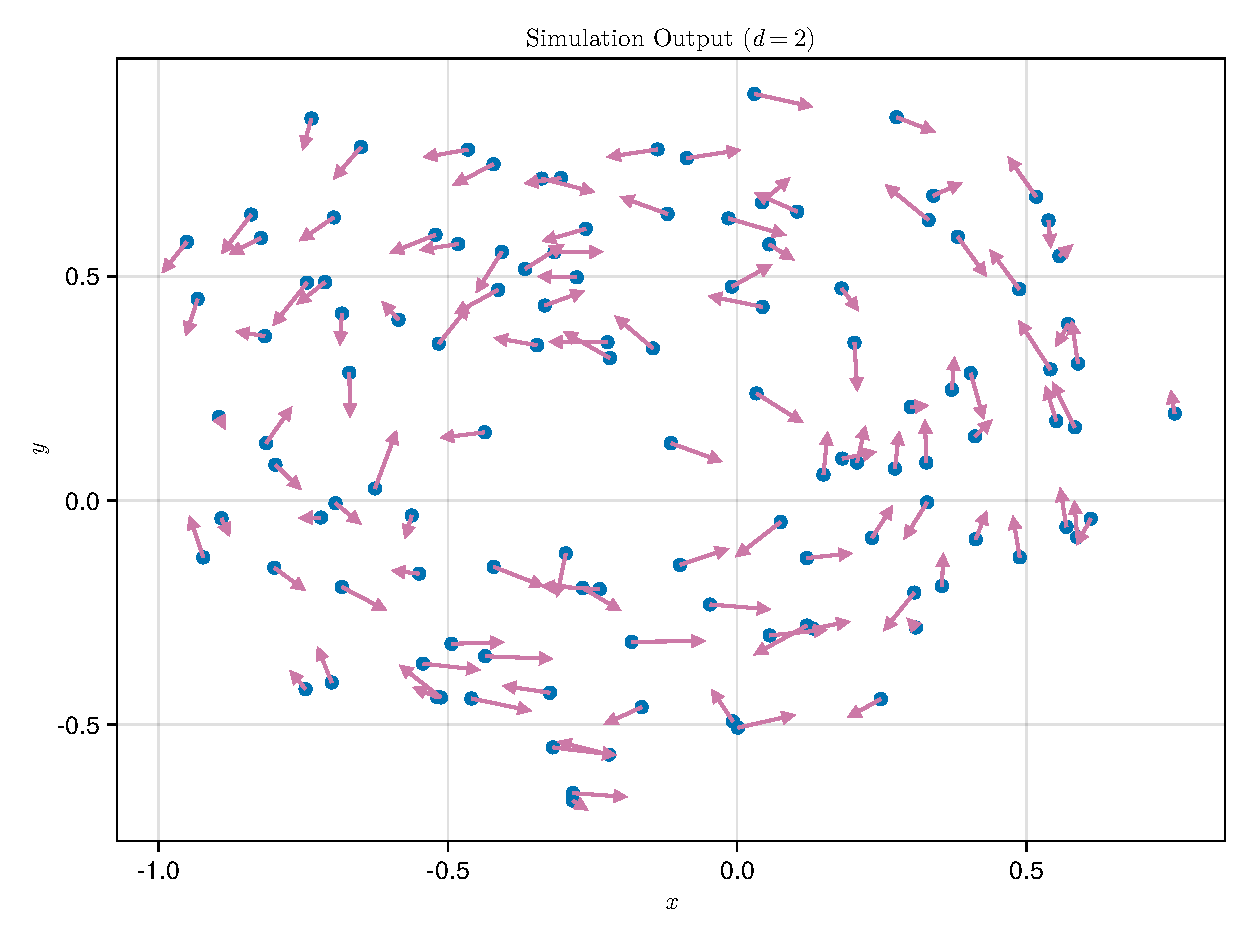
\includegraphics[width=0.8\linewidth]{results/morse-2d/simulation-quiver.pdf}
  \caption[Quiver plot of 120 particles in 2D interacting through the Morse potential]{Position and velocity of $N_p = 120$ particles $d = 2$ dimensions as obtained through the molecular dynamics simulation introduced in \Cref{chap:particle-simulator}. The interaction potential is a Morse potential with given parameters. Friction and self-propulsion terms are present as described in \cite{2006-self-propelled}, so using $f(v_i) = 1.6 - 0.5 v_i^2$, this figure reproduces their results.}
  \label{fig:simulation-quiver-illustration}
\end{figure}

% TODO: Friction Term -> Energy Dissipation -> Different Plot

\section{Kinetic Theory: The Vlasov Equation}
A very common tool in Plasma physics.
$$\frac{\partial f}{\partial t}+{\frac {\mathrm {d} \mathbf {r} }{\mathrm {d} t}}\cdot {\frac {\partial f}{\partial \mathbf {r} }}+{\frac {\mathrm {d} \mathbf {p} }{\mathrm {d} t}}\cdot {\frac {\partial f}{\partial \mathbf {p} }}=0,$$

This is the collisionless Boltzmann equation.
Vlasov replaces the collision term with long-range interactions.

\begin{theorem}{Liouville's}{liouville}
  Says that phase-space volume is conserved in situations of a pure particle-particle interaction.
  $$\frac{d\hat{\rho}}{dt}=
    \frac{\partial\hat{\rho}}{\partial t}
    +\sum_{i=1}^n\left(\frac{\partial\hat{\rho}}{\partial q_i}\dot{q}_i
    +\frac{\partial\hat{\rho}}{\partial p_i}\dot{p}_i\right)=0\,.$$
\end{theorem}

\section{Vicsek Model}
For the study of active matter (a number of individual agents).
\hierKoennteIhreWerbungStehen

\section{Swarming in Biological Settings}
A 2010 paper by \citeauthor{2010-starlings} showed the surprising result that correlation between movement of individual starlings in bird flocks over Rome is scale-free.
In contrast to the assumption that birds only mirror their neighbours' behaviour and swarming behaviour emerges as a result of that, this observation suggests that bird flocks exert collective behaviour beyond local interactions.
\begin{quote}
  The change in the behavioural state of one animal affects and is affected by that of all other animals in the group, no matter how large the group is
  \parencite{2010-starlings}.
\end{quote}
This work was done by individually tracking each starling in the flock and using tracking algorithms to represent their 3 dimensional positions and velocities.

\section{Analytical Solutions}
\label{sec:analytical-solutions}
\cite{2017-explicit-solutions} provides some analytic solutions to \hyperref[def:the-problem]{the problem}.
For example with an attractive-repulsive potential as given in \Cref{eq:attractive-repulsive-potential}, when $\alpha = 2$ and $\beta \in [-1, 2]$, the equilibrium measure is given by
\begin{equation}
  \hat{\rho}(\hatvec{x}) = C_\beta \cdot R^d \cdot \left(R^2 - \hatvec{x}^2\right)^{\frac{1-\beta}{2}}\,,
  \label{eq:analytical-solution-alpha-equal-2}
\end{equation}
where
$$C_\beta := \frac{1}{(\beta - 1) \pi} \cos\left(\frac{(2 - \beta) \pi}{2}\right)\,,$$
$$R := \left(C_\beta \cdot B\left(\frac{1}{2}, \frac{3 - \beta}{2}\right)\right)^{\frac{1}{\beta - 2}}\,,$$
with $B(\cdot, \cdot)$ the beta-function (cf. \Cref{def:beta-function}).

% TODO: is this only 1-d or n-d?
% TODO: the R^d is my own extension - can we prove?

  \chapter{Particle Simulator}
\label{chap:particle-simulator}

While local behaviour may be according to simple rules, the aforementioned many-body systems generally exhibit complex behaviour when viewed as a whole.
This behaviour can be captured in mathematical terms but also from a simulation perspective.
Particle simulations such as the ones depicted in \Cref{fig:simulation-quiver,fig:morse-3d-quiver} are well-studied in physics and scientific computing more generally.
This class of simulations, in the context of intermolecular interactions, is often referred to as molecular dynamics.

\begin{figure}[H]
  \centering
  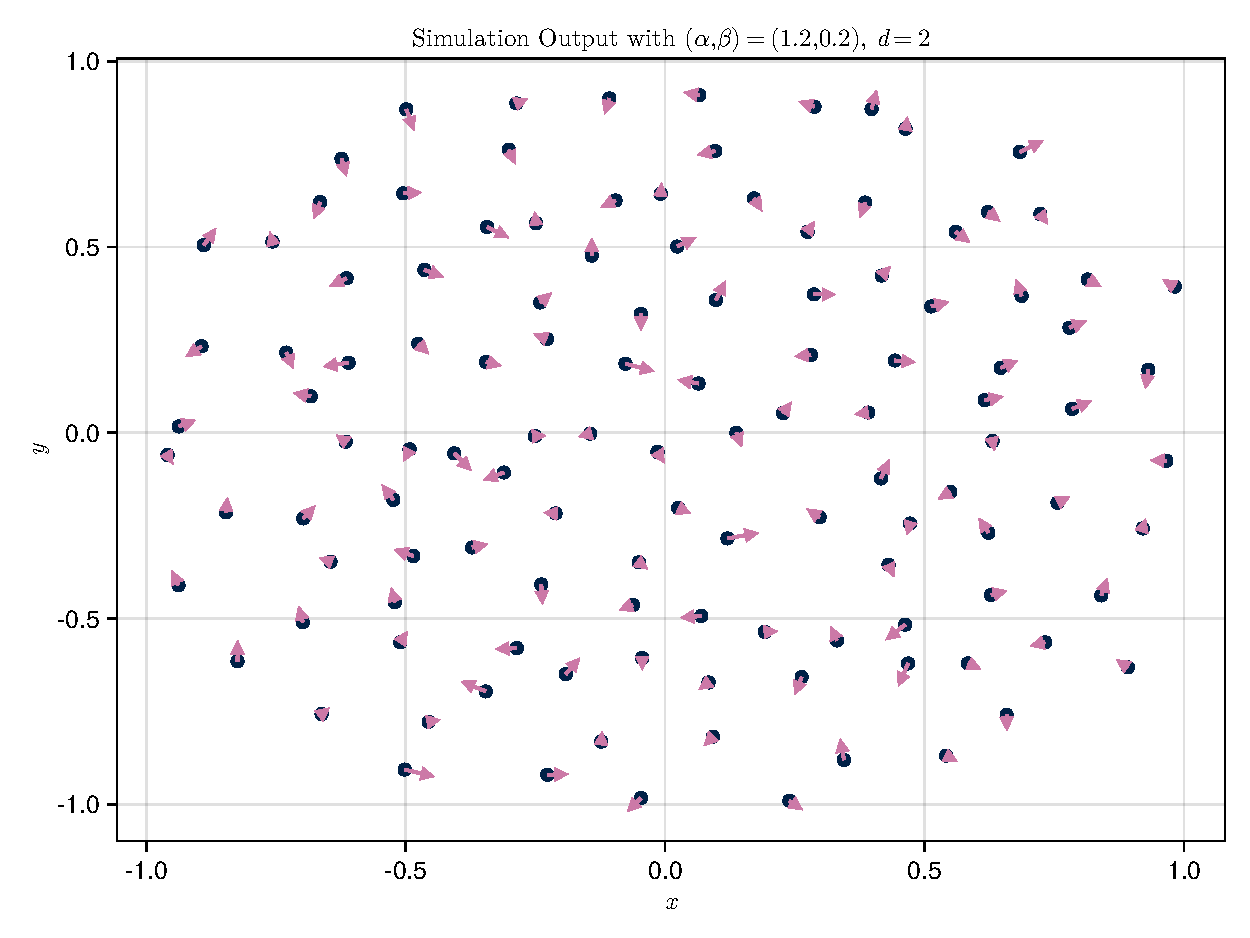
\includegraphics[width=0.72\linewidth]{results/known-2d/simulation-quiver.pdf}
  \caption[Quiver plot of 120 particles in 2D interacting through the attractive-repulsive potential]{Position and velocity of particles in the simulation at a point in time. Every particle, each of equal mass $m$, interacts with every other particle through the interaction potential $U_{ij} = K\left(\norm{\vec{x_i} - \vec{x_j}}\right)$ leading to $\mathcal{O}(N_p^2)$ interactions.}
  \label{fig:simulation-quiver}
\end{figure}

Because each particle interacts with every other particle, the number of interactions scales with $\mathcal{O}(N_p^2)$,
which can play a prohibitive role in terms of the computation time when increasing the number of particles $N_p \gg 1$.

Within the scope of this thesis, in order to understand the elaborate behaviour of such particle systems and also to verify results from theory and the spectral method, we provide an implementation of a simulator starting from a numerical time integrator in $\R^d$.
In addition to the \textit{headless} simulation software, exporting state and results for treatment by the analysis component, a \gls{gui} is provided to enable live insight into and interaction with the model, cf. \Cref{fig:gui-screenshot}.

\begin{figure}[H]
  \centering
  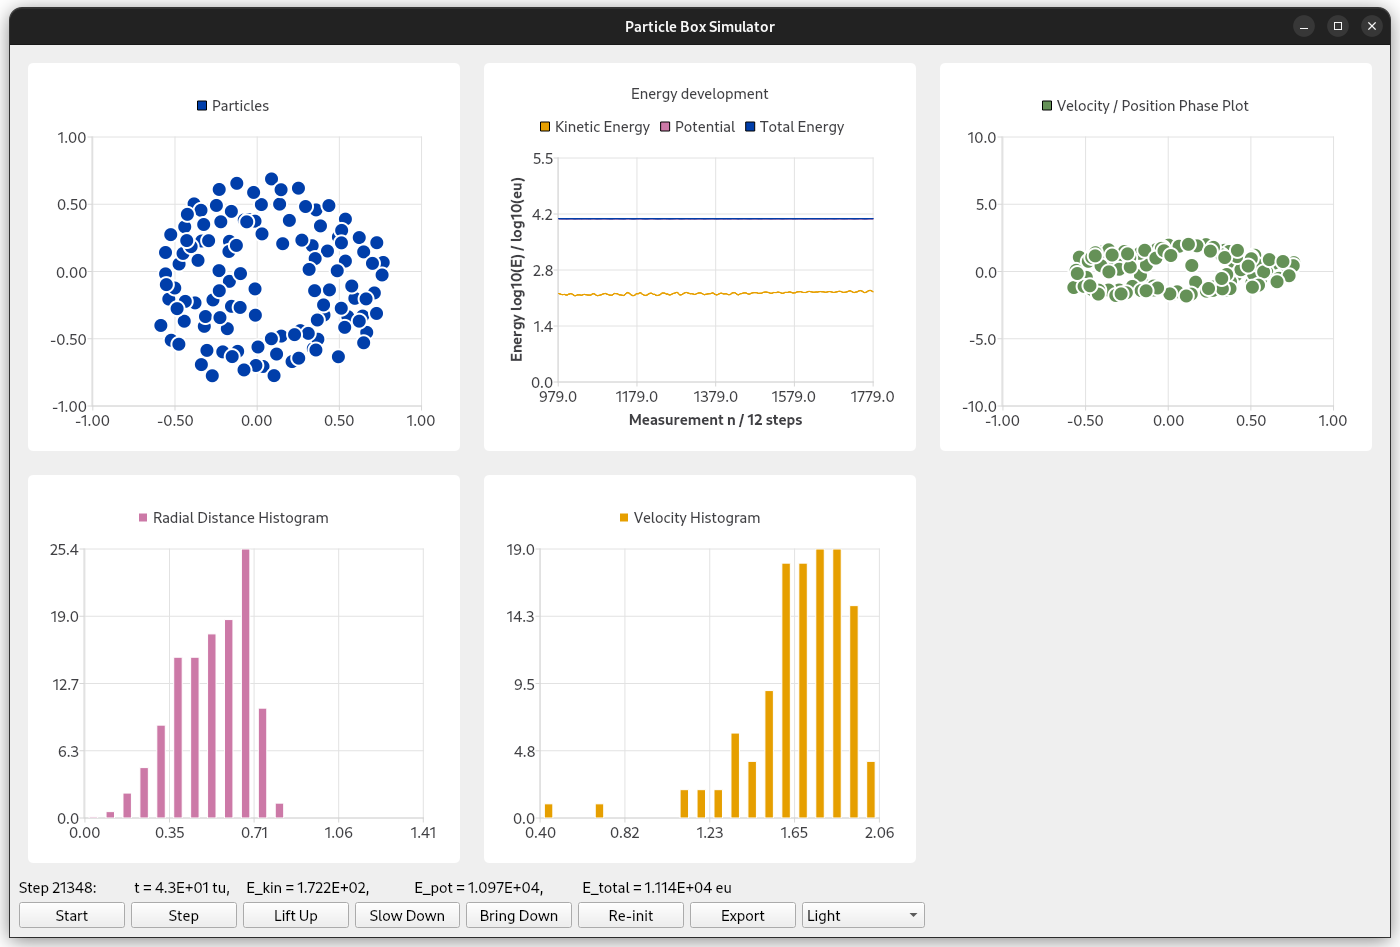
\includegraphics[width=\linewidth]{gui-screenshot.png}
  \caption[Graphical User Interface of the Simulator]{Screenshot of the \gls{gui} provided for the particle simulator. The top row shows the position of particles in their $[-1, 1]^d$ ($d = 2$ in this case) domain at a point $t$ in time, the energy development over time and the current position/velocity phase space plot. Below, there are position and velocity histogram updated live along with the simulation.}
  \label{fig:gui-screenshot}
\end{figure}

\begin{figure}[H]
  \centering
  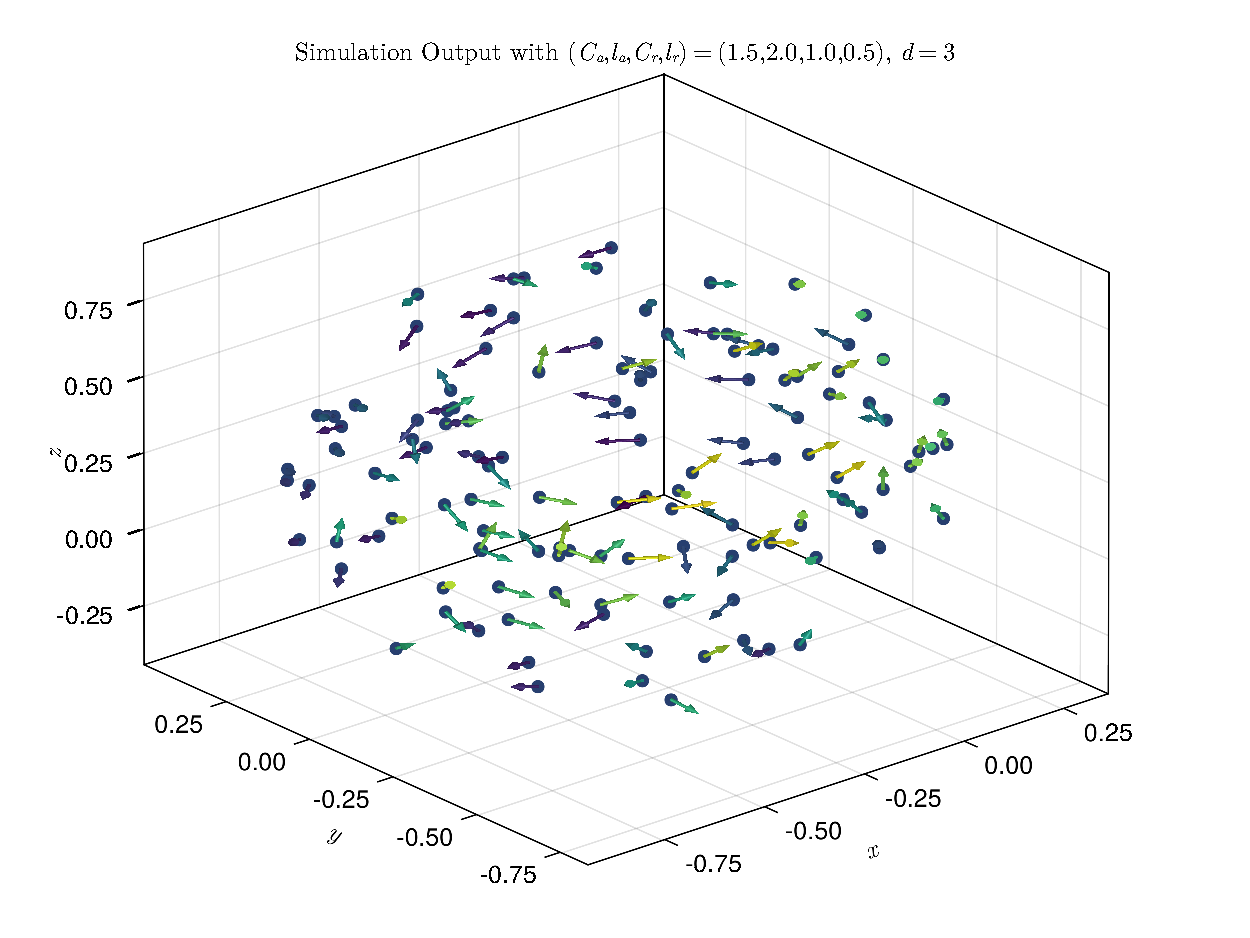
\includegraphics[width=0.8\linewidth]{results/morse-3d/simulation-quiver-3d.pdf}
  \caption[Self-propelled particles in 3D interacting through $K_{C_a, l_a, C_r, l_r}(r)$.]{Self-propelled particles in a reflective box $[-1, 1]^3$ interacting via the Morse potential $K_{C_a, l_a, C_r, l_r}(r)$ in $d=3$ dimensions.}
  \label{fig:morse-3d-quiver}
\end{figure}

\section{Available Methods}
As a particular important problem in the physical sciences, there is an abundant number of simulation methods and solvers available for molecular dynamics problems.

Among them are simple forward integrators (e.g. $\vec{x_i}(t + \tau) \approx \vec{x_i}(t) + \tau \vec{v_i}(t)$ for $t > 0$ and timestep $\tau \in \R^+$), a generalisation of which are multistep methods.
Both essentially originate from expanding the position and velocity as Taylor series in time.
They work well in many general cases and error analysis is straightforward.

Named within the ``Top 10 Algorithms of the 20th Century'' \parencite{2000-top-algorithms}, the \gls{fmm} due to \cite{1987-multipole-method} uses a multipole expansion of the system's Green's function to cluster together interactions with far-away particles for physical interaction potentials such as the Coulomb- or gravitational potentials.
It does so by hierarchically clustering together particles based on position and treating interaction with far-away particles as a single interaction, therefore reducing the runtime from $\mathcal{O}(N_p^2)$ for each pair of particles down to $\mathcal{O}(N_p)$.
\gls{fmm} is among the few methods with rigorous results available on the error.
For long-range interactions however, as they are ubiquitous within this thesis (cf. the summary in \Cref{fig:comparing-potentials}), the \gls{fmm} is not applicable.

Another specialised method for the integration of Newton's equations of motion is leapfrog integration, our method of choice for the C++ implementation of the $N_p$-body simulator.

\subsection{Leapfrog Integration}
The Leapfrog algorithm is a more effective forward integration method due to its high resistance to numerical round-off error.
Except for minor changes in the way the velocity is updated, it is essentially the same as the velocity Verlet algorithm, a variant of Verlet integration with error on the order of $\mathcal{O}(\tau^4)$ with $\tau \in \R^+$ the timestep.

In particular, every particle $i$ at position $\vec{x_i} \in \R^d$ with velocity $\vec{v_i} \in \R^d$ is updated using
\begin{align*}
  \vec{x_i}(t+\tau)     & = \vec{x_i}(t)+\tau \cdot \vec{v_i}(t+\tau / 2),              & \quad\text{for}~ & t=0, \tau, \ldots\,,      \\
  \vec{v_i}(t+\tau / 2) & = \vec{v_i}(t-\tau/2) + \tau \cdot \vec{f}[\vec{x_i}(t), t],  & \quad\text{for}~ & t=\tau, 2 \tau, \ldots\,, \\
  \vec{v_i}(\tau / 2)   & = \vec{v_i}(0)+\frac{\tau}{2} \cdot \vec{f}[\vec{x_i}(0), 0], & \quad\text{for}~ & t=0\,,
\end{align*}
where $\vec{f_i}[\vec{x_i}(t), t] \in \R^d$ denotes the acceleration (sum of contributions of all forces divided by particle mass $m_i$).
Verlet integration methods are a common technique in molecular dynamics for the integration of Newton's equations of motion and implemented in many solvers.
Leapfrog integration can be improved to higher accuracy using Yoshida coefficients \parencite{1973-yoshida-coefficients}.
% TODO: vielleicht eine kleine Figure zur Visualisierung des Leap-Frogs
Our implementation can be found in \Cref{appendix:code-snippets}.

% TODO: where we note that $\nabla f(\norm{\vec{x}}) = \frac{\vec{x}}{\norm{\vec{x}}} f'(\norm{\vec{x}})$.

\section{Phase Space}
Each particle, at every point in time $t$, has a position and velocity value.
In $d=1$ dimension, one can visualise both of these quantities simultaneously in a phase space plot (cf. \Cref{fig:phase-space-plot}).
For $d > 1$ dimension, it is possible to either only visualise the first components $\{\vec{x_i}\}_1$ and $\{\vec{v_i}\}_1$ or to visualise the norm of the position (distance from the centre of mass) $r = \norm{\vec{x_i} - \vec{x}_{\text{centre}}}$ and velocity $\norm{\vec{v_i}}$.

\begin{figure}[H]
  \centering
  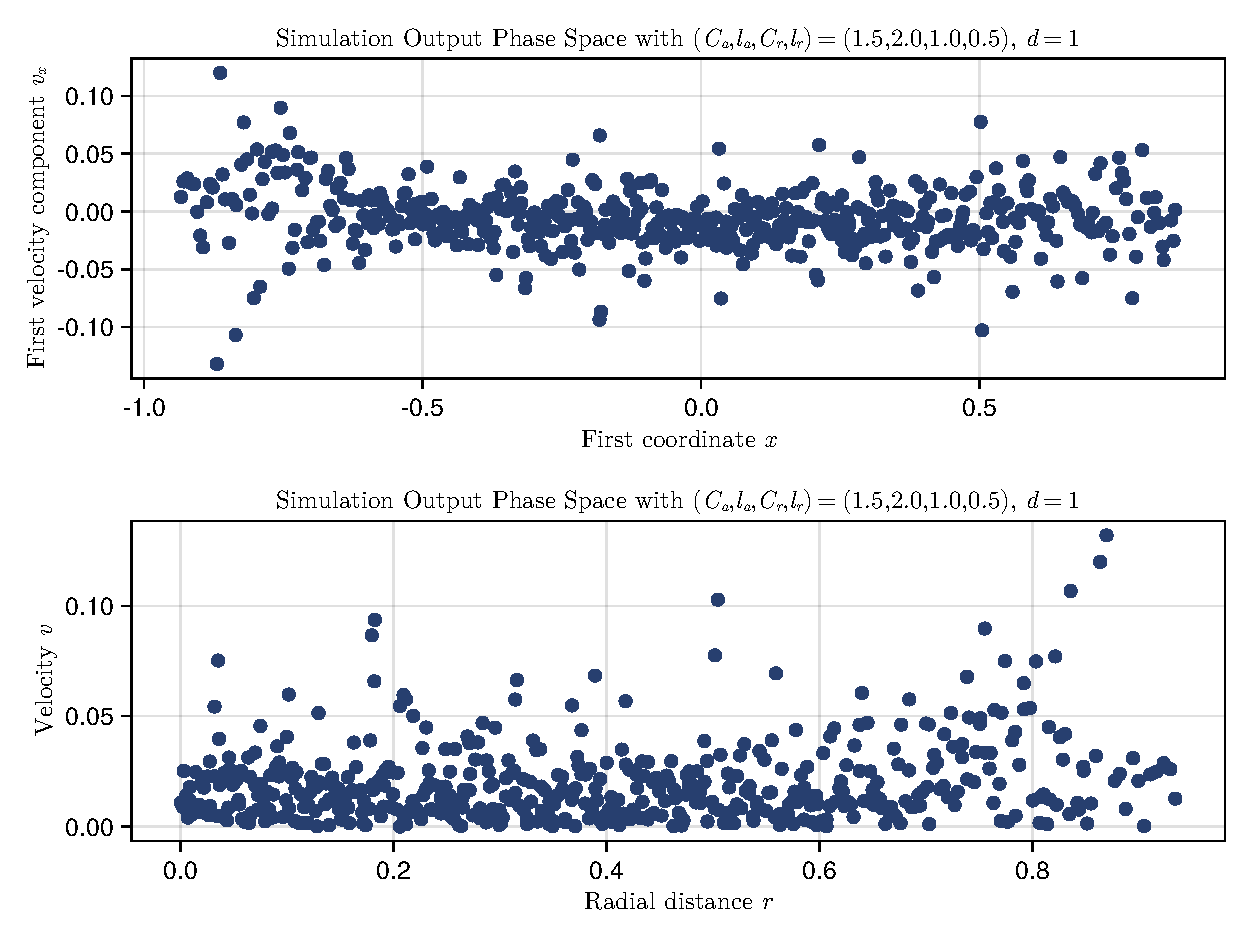
\includegraphics[width=0.8\linewidth]{results/morse/phase-space-plot.pdf}
  \caption[Phase Space Plots]{Position and velocity of $N_p = 500$ particles in a $d=1$ simulation visualised as phase space plots using the two different visualisation mechanisms. In the top plot, one can observe natural rotation around the origin $(0, 0)$ as positive velocity corresponds to movement to the right and negative velocity to leftwards movement. The color indicates the $x$-coordinate of the particle, respectively (shown to visualise correspondence between the upper and the lower plot).}
  \label{fig:phase-space-plot}
\end{figure}

The behaviour of the phase space plot differs from potential to potential, most importantly one can observe multiple centers of rotation for the Morse potential in addition to the origin, whereas an attractive-repulsive potential builds up to an elliptical shape in the phase space plot.
% TODO: why is this? Local interactions?

\begin{figure}[H]
  \centering
  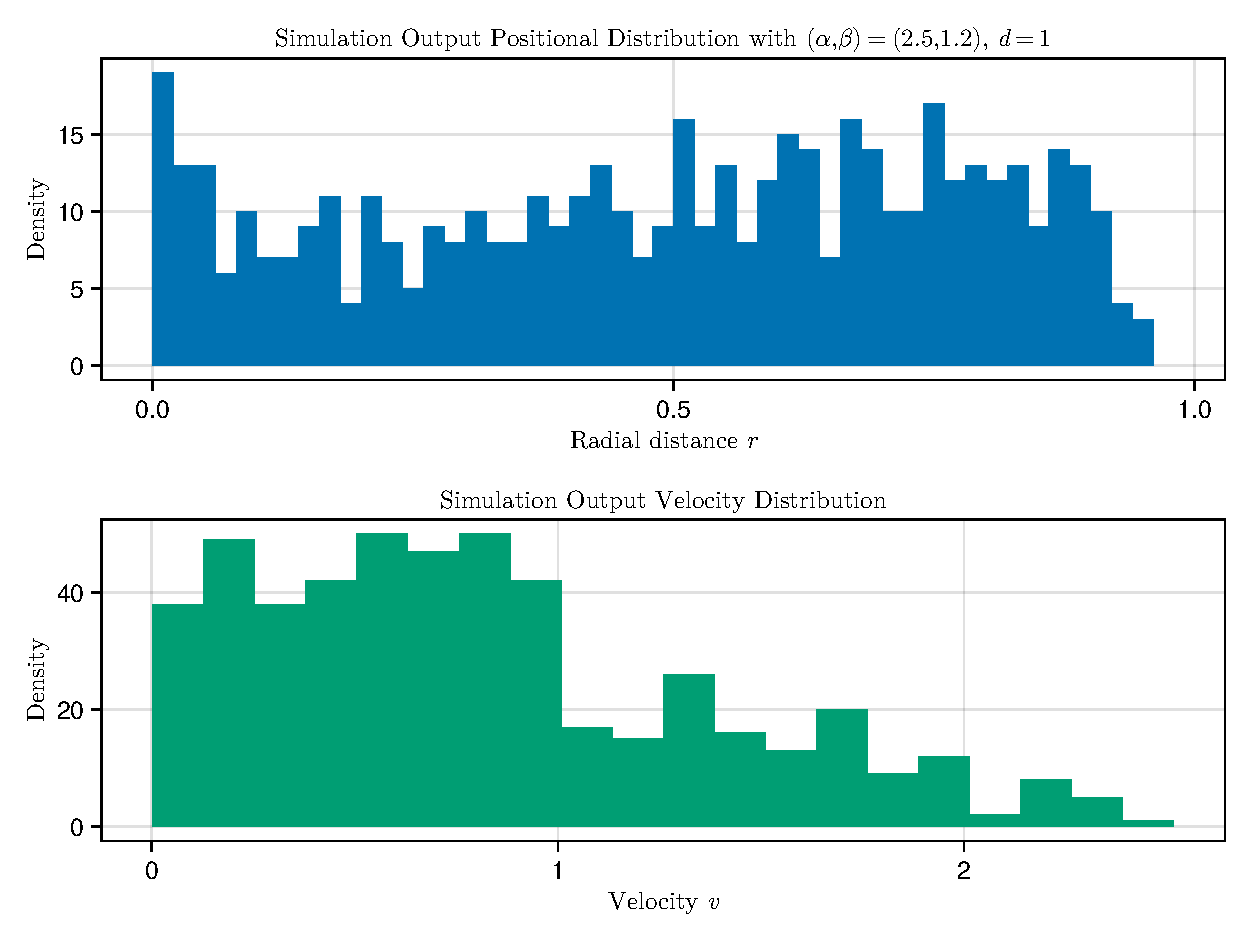
\includegraphics[width=0.8\linewidth]{results/attrep/simulation-histogram.pdf}
  \caption[Radial Distance and Velocity Histograms of attractive-repulsive Simulation Output in 1D]{Radial Distance ($r$) and Velocity ($v$) Histograms as obtained through a long-running simulation of $N_p = 500$ particles interacting through an attractive-repulsive potential $K_{\alpha, \beta}(r)$. The spectral method introduced in \Cref{chap:spectral-method} aims to solve for the particle density as a function of radial distance, hoping to predict the shape of the positional histogram.}
  \label{fig:simulation-histogram}
\end{figure}

In a physical setting with collision terms, the velocity distribution $f(\hat{v})$ would approach the shape of a Boltzmann distribution
$$f(\hat{v})={\bigg(\frac{m}{2\pi k_B T}\bigg)}^{\frac {3}{2}}\,4\pi \hat{v}^{2}\exp \left(-{\frac {m \hat{v}^{2}}{2k_B T}}\right)\,,$$
with $m$ the identical mass of each particle and velocity $\hat{v}$, $k_B$ the Boltzmann constant and $T \in \R^+$ is temperature, measured in Kelvin.
An exemplary velocity distribution is given in \Cref{fig:simulation-histogram}.

\section{Runtime Analysis}
\hierKoennteIhreWerbungStehen

\section{Further Experiments}
One can obtain interesting patterns using the absolute-value potential $K_{||}(r)$ as given in \Cref{eq:absvalue-potential} in $d=3$ dimensions, cf. \Cref{fig:gyroscope-quiver-3d,fig:fcc-quiver-3d}.
Because $K_{||}(r)$ is not continuously differentiable, the potential is not at all physical.
However, due to its linear penalty (instead of exponentials or power laws) it allows for a wider range of intriguing shapes of the collection of particles.

\begin{figure}[H]
  \centering
  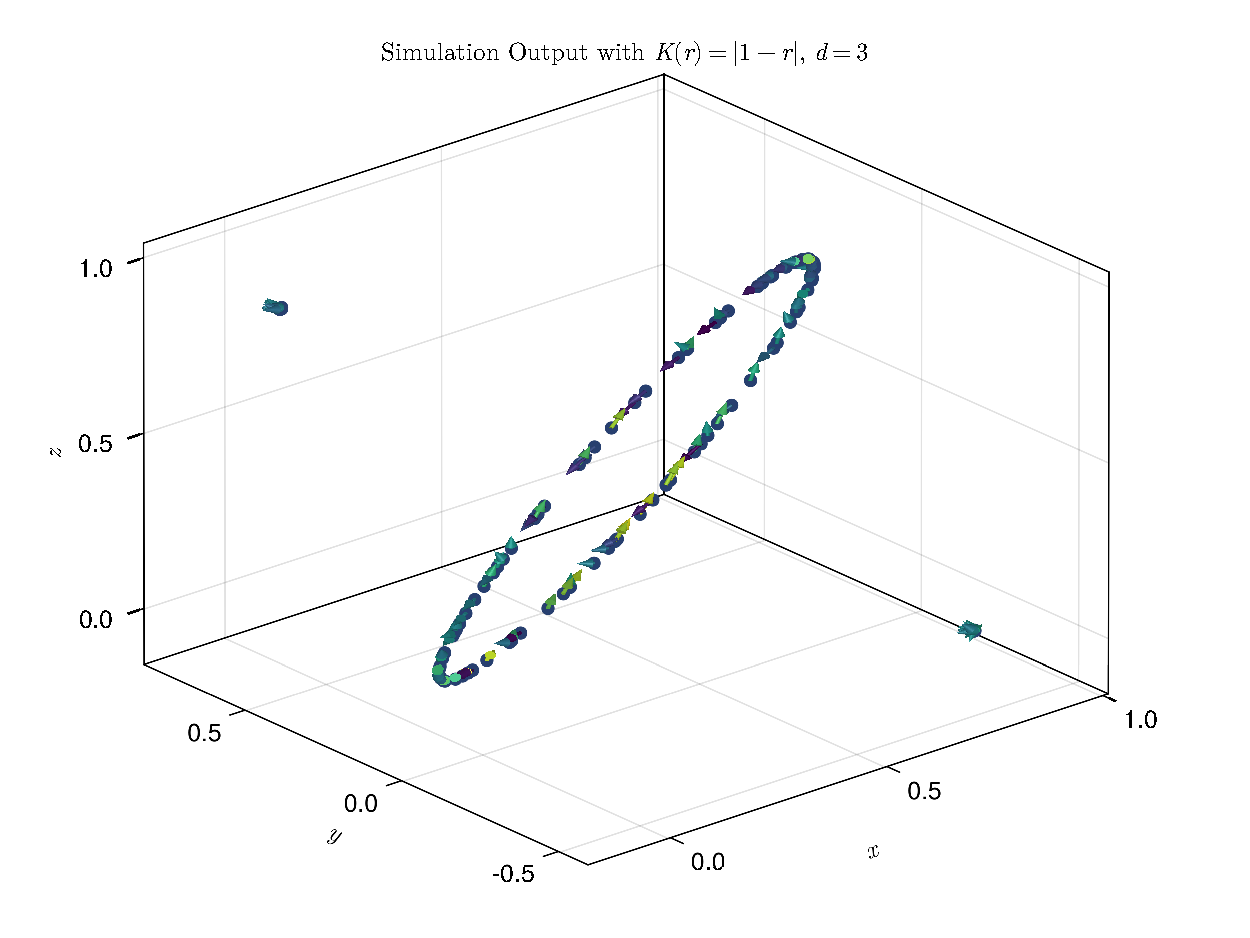
\includegraphics[width=0.8\linewidth]{results/gyroscope-3d/simulation-quiver-3d.pdf}
  \caption{When running with $K(r) = |1-r|$ as an interaction potential and hence, $F(r) = -\nabla K(r) = -\sign(1-r)$, in $d=3$ dimensions a gyroscopical shape will form. The two outlying points are actually many particles above one another (high concentration of mass) and they form the axis of the rotating circle of particles.}
  \label{fig:gyroscope-quiver-3d}
\end{figure}

\begin{figure}[H]
  \centering
  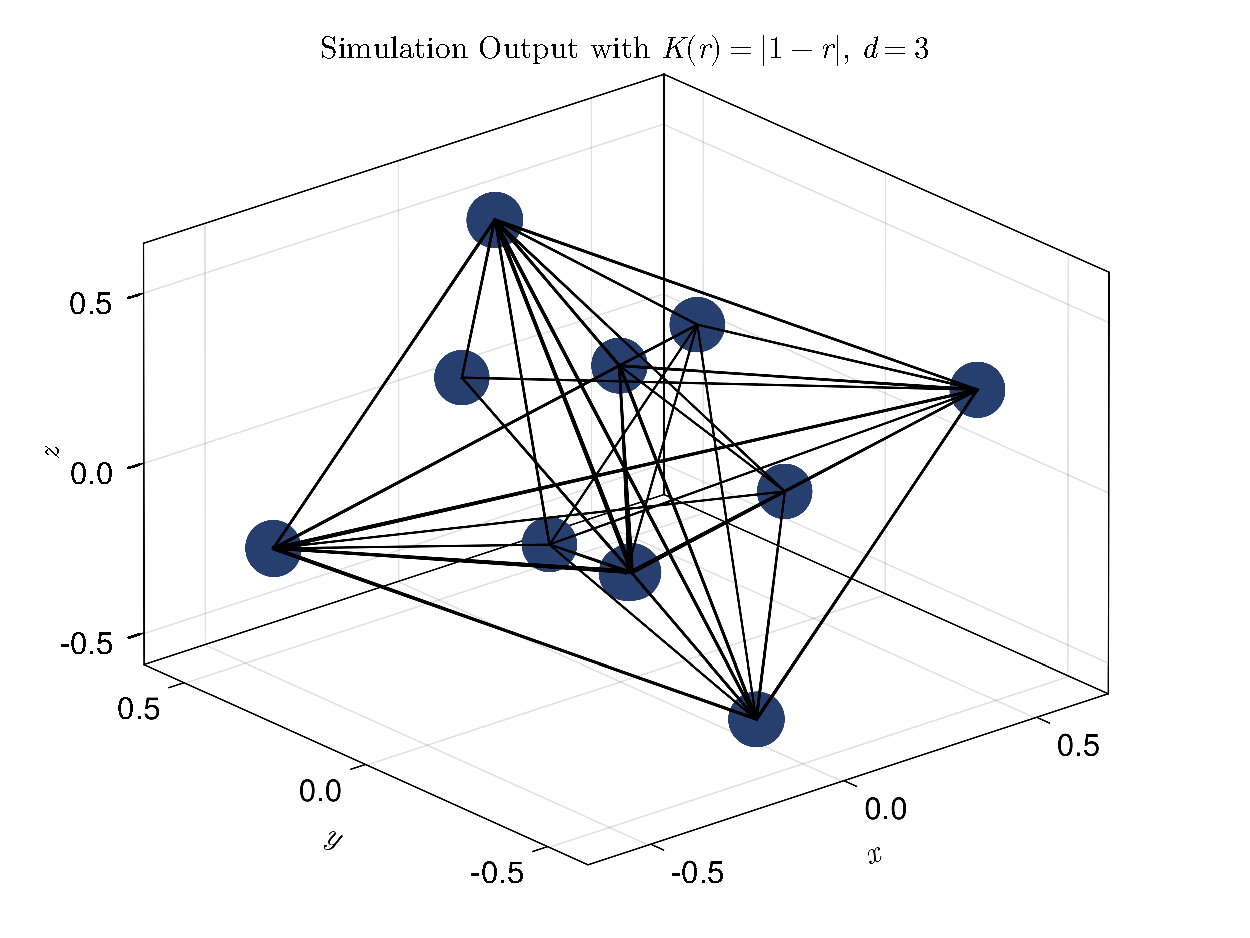
\includegraphics[width=0.8\linewidth]{results/gyroscope-3d/simulation-fcc-3d.pdf}
  \caption{When running an $N_p = 250$ particle simulation with $K(r) = |1-r|$ as an interaction potential in $d=3$ dimensions the particles will align into a stable ``optimal packing'' arrangement. In this case, they approximate a \gls{fcc} array of spheres, potentially providing a starting point for other algorithms.}
  \label{fig:fcc-quiver-3d}
\end{figure}

% TODO: add more details on the optimal packing? Maybe that this could be developed into an actual algorithm, etc.?

  \chapter{Spectral Method}
\label{chap:spectral-method}

% \section{Content}
% \input{chapters/out/Spectral Method.md.tex}

\section{Definitions}
\begin{definition}{Rising Factorial (Pochhammer Symbol)}{rising-factorial}
  The $n$th rising factorial of $x \in \R$ is given by
  $$(x)_n := \prod_{k=0}^{n-1} (x+k) \,\in \R\,.$$
\end{definition}

For example, $(3.141)_5 = 3.141 \cdot 4.141 \cdot 5.141 \cdot 6.141 \cdot 7.141$.

\begin{remark}{Nonpositive integer rising factorial}{nonpositive-pochhammer}
  When the argument is a nonpositive integer, the rising factorial
  $(-m)_n = -m \cdot (-m+1) \cdot ... \cdot (-m+n-1)$
  vanishes when $n \ge m+1$ for $n \in \N$ and $m \in \N_0$ as $0$ is among the factors.
\end{remark}

\begin{definition}{Orthogonal Polynomials}{orthogonal-polynomials}
  Are univariate polynomials
  $$p_n: \R \mapsto \R, \; p_n(x) = \sum_{k=0}^{n} c_k x^k\,.$$
  that form an orthogonal basis under some inner product $\langle p_n, p_m \rangle_w$ with weight function $w(x)$, given by
  $$\langle f, g \rangle_w := \int_{-1}^{1} f(x) g(x) w(x) \,\ddx\,.$$
\end{definition}

\begin{remark}{}{symmetry-of-inner-product}
  The inner product satisfies $\langle x\mapsto xf(x), g \rangle_w = \langle f, x \mapsto xg(x)\rangle_w$.
\end{remark}

\begin{theorem}{Three-Term Recurrence Relationship}{three-term-recurrence-relationship}
  All orthogonal polynomials $\{p_0, p_1, p_2, ...\}$ (cf. \Cref{def:orthogonal-polynomials}) have (at least) a three-term recurrence relationship of the form
  $$A_n p_{n+1}(x) = B_n p_n(x) + C_n p_{n-1}(x)\,.$$
\end{theorem}
\begin{proof}
  Consider ``$x p_n$''$:= x \mapsto x p_n(x)$, a polynomial with $\deg(x p_n) \le n+1$.
  By the linear independence of all orthogonal polynomials $p_n$ with respect to the inner product $\langle \cdot, \cdot \rangle_w$, it must be possible to write
  $$x p_n(x) = \sum_{k=0}^{n+1} \hat{a}_k p_k(x)\,,\quad \text{for some}~\hat{a}_k \in \R, k=0, ..., n+1\,.$$
  Now, for all $n \ge 0$ and $m \le n+1$ we have
  $$\langle xp_n, p_m \rangle_w = \sum_{k=0}^{n+1} \hat{a}_k \langle p_k, p_m \rangle_w = \sum_{k=0}^{n+1} \hat{a}_k \delta_{i,k} = \hat{a}_m \langle p_m, p_m \rangle_w\,,$$
  due to the orthogonality relationship (\Cref{thm:jacobi-orthogonality-condition}).
  Therefore,
  \begin{equation}
    \hat{a}_m = \frac{\langle xp_n, p_m \rangle_w}{\langle p_m, p_m \rangle_w} \quad\text{for all}~m \le n+1\,.
    \label{eq:three-term-step}
  \end{equation}

  But when \underline{$m < n-1$}, we have $\deg(xp_m) < n$ so $x p_m(x) = \sum_{k=0}^{n-1} \hat{b}_k p_k(x)$ for some (potentially 0) $\hat{b}_k \in \R$, and therefore $\langle p_n, xp_m \rangle_w = \sum_{k=0}^{n-1} \hat{b}_k \langle p_n, p_k \rangle_w = 0$,
  which, by the symmetry of the inner product (\Cref{remark:symmetry-of-inner-product}), also implies $\langle x p_n, p_m \rangle_w = 0$ which, by \Cref{eq:three-term-step}, allows us to conclude that the earlier coefficients $\hat{a}_m = 0$.

  % And obviously, even if we assumed higher-order coefficients in the expansion of $xp_n$, when $m > n+1 \Leftrightarrow n < m-1$, $\deg(xp_n) < m$ and so all later coefficients $\hat{a}_m = 0$.

  We recall that $xp_n(x) = \sum_{k=0}^{n+1} \hat{a}_k p_k(x)$, which in combination with our insights on the $\hat{a}_m$ above means that
  $$xp_n(x) = \hat{a}_{n-1} p_{n-1}(x) + \hat{a}_{n} p_n(x) + \hat{a}_{n+1} p_{n+1}(x)\,,$$
  concluding the proof.
\end{proof}

For example, for the Chebyshev polynomials (cf. \Cref{def:chebyshev-polynomials}) we have
$$T_{k+1}(x) = 2x T_k(x) - T_{k-1}(x) \,.$$

% From HeatFun:
% \begin{theorem}{Chebyshev recursion formula}{chebrecursion}
%   The \chebyshev polyomials satisfy the three-term recurrence relation $$T_{k+1}(x) = 2x T_k(x) - T_{k-1}(x) \,.$$
% \end{theorem}
% \begin{proof}{\parencite{atap}.}
%   For $k > 1$, we have
%   \begin{align*}
%     2x T_k(x) - T_{k-1}(x) & = 2x \cdot \frac{1}{2} (z^k + z^{-k}) - \frac{1}{2} (z^{k-1} + z^{-(k-1)})                     \\
%                            & = 2 \frac{1}{2}(z + z^{-1}) \cdot \frac{1}{2}(z^k + z^{-k}) - \frac{1}{2} (z^{k-1} + z^{-k+1}) \\
%                            & = \frac{1}{2} (z^{k+1} + z^{k-1} + z^{-k+1} + z^{-k-1}) - \frac{1}{2} (z^{k-1} + z^{-k+1})     \\
%                            & = \frac{1}{2} (z^{k+1} + z^{-(k+1)}) = T_{k+1}(x)
%   \end{align*}
% \end{proof}

\begin{definition}{Generalised Hypergeometric Series}{generalised-hypergeometric-series}
  The generalised hypergeometric series ${}_pF_q: \R^p \times \R^q \times \C \mapsto \C$ with $p, q \in \N$ is defined by
  $${}_2F_1\left(\begin{matrix}a_{1}, \ldots, a_{p} \\b_{1}, \ldots, b_{q}\end{matrix}; z\right) := \sum _{k=0}^{\infty }{\frac {(a_{1})_{k}\cdots (a_{p})_{k}}{(b_{1})_{k}\cdots (b_{q})_{k}}}\,{\frac {z^{k}}{k!}}\,,$$
  where $(\cdot)_k$ denotes the rising factorial (cf. \Cref{def:rising-factorial}).
\end{definition}

Note that any permutation of the first (``top'') arguments $a_1, ..., a_p$ leaves the function unchanged due to commutativity of multiplication on $\C$. The same holds for the second (``bottom'') arguments $b_1, ..., b_q$.

\begin{lemma}{Gaussian Hypergeometric Function}{gaussian-hypergeometric-function}
  The $p=2$, $q=1$ special case of the generalised hypergeometric series can also be evaluated by
  $${}_2F_1\left(\begin{matrix}a_{1}, -n \\b_{1}\end{matrix}; z\right) = \sum_{k=0}^n (-1)^k \binom{n}{k} \frac{(a_1)_k}{(b_1)_k}z^k\,,$$
  when the second argument $a_2 = -n$ is a nonpositive integer, so $n \in \N_0$.
\end{lemma}
\begin{proof}
  Starting from the definition of the generalised hypergeometric series ${}_pF_q$ with $p=2$ and $q=1$ (\Cref{def:generalised-hypergeometric-series}),
  $${}_2F_1\left(\begin{matrix}a_{1}, -n \\b_{1}\end{matrix}; z\right) = \sum_{k=0}^{\infty} \frac{(a_1)_k (-n)_k}{(b_1)_k} \frac{z^k}{k!} = \sum_{k=0}^{n} \frac{(a_1)_k (-n)_k}{(b_1)_k} \frac{z^k}{k!}\,,$$
  which can be terminated at $k=n$ due to \Cref{remark:nonpositive-pochhammer}, we can express
  $$\frac{(-n)_k}{k!} = \binom{-n+k-1}{k} = (-1)^k \binom{1+n-k+k-1}{k} = (-1)^k \binom{n}{k}$$
  using a well-known relation between the Pochhammer symbol and the binomial coefficient which immediately leads us to  % TODO: where can one find this well-known relation?
  $${}_2F_1\left(\begin{matrix}a_{1}, -n \\b_{1}\end{matrix}; z\right) = \sum_{k=0}^n \binom{n}{k} \frac{(a_1)_k}{(b_1)_k}(-z)^k\,,$$
  concluding the proof.
\end{proof}

Note that these functions are generally tricky to evaluate efficiently, recent advancements have enabled their usage in a broader range of applications \parencite{2008-hypergeometric-functions-jl-1,2017-hypergeometric-functions-jl-2,2023-hypergeometric-functions-jl-3}.
Implementations are available in the \href{https://github.com/JuliaMath/HypergeometricFunctions.jl}{HypergeometricFunctions.jl} package in Julia.

More details on the Gaussian hypergeometric series, sometimes simply referred to as the hypergeometric function, its defining differential equation origin, modular interpretations and symmetries may be found in the 1997 book \citetitle{1997-hypergeometric-functions-my-love} \parencite{1997-hypergeometric-functions-my-love}.

\begin{definition}{Jacobi Polynomials}{jacobi-polynomials}
  Let $P^{(a, b)}: \C \mapsto \C$ with
  $$P^{(a,b)}_n(x) = {\frac{(a +1)_{n}}{n!}}\,{}_{2}F_{1}\left(-n,1+a +b +n;a +1;{\tfrac  {1}{2}}(1-x)\right)$$
  So are defined using the Gaussian Hypergeometric Function (cf. \Cref{def:gaussian-hypergeometric-function}) and the Pochhammer symbol.
  Which is equivalent to
  $$P_{n}^{{(a, b)}}(x)={\frac  {\Gamma (a +n+1)}{n!\,\Gamma (a +b +n+1)}}\sum _{{m=0}}^{n}\binom{n}{m}{\frac{\Gamma (a +b +n+m+1)}{\Gamma (a +m+1)}}\left({\frac{x-1}{2}}\right)^{m}\,.$$
  where $\Gamma (x)=\int _{0}^{\infty }t^{x-1}e^{-t}\,\ddt$ (with $\Re(x)>0$) is the gamma function \footnote{Recall that for integer arguments $k \in \N$, it equals the factorial of $(k-1)$ so $\Gamma(k) = (k-1)!$.}.

  Gegenbauer Polynomials (cf. \Cref{def:gegenbauer-polynomials}) are a special case. And
  Chebyshev Polynomials (cf. \Cref{def:chebyshev-polynomials}) are a special case of them.
\end{definition}

Following from this definition,
\begin{align*}
  P_0^{(a, b)}(x)   & = 1                            \\
  P_{1}^{(a, b)}(x) & = (a+1)+(a+b+2){\frac{x-1}{2}}
\end{align*}
and so on. Note that obviously, $\deg\left(P_k^{(a, b)}\right) = k$.

Nice Spectral Properties:
\begin{itemize}
  \item Differentiation
  \item Three-Term Recurrence
  \item why are they better than just Chebyshev?
\end{itemize}

Note that in this manuscript we will use the dot-product notation
$$f(x) = \sum_{k=0}^{N-1} f_k P_k^{(a, b)}(x) \qLRq f(x) = \vec{f} \cdot \vec{P}^{(a, b)}(x)\,,$$
to express that a function $f$ is a linear combination of basis polynomials with coefficients $\vec{f} = (f_0, ..., f_{N-1})^T \in \R^N$.
So $\vec{P}^{(a, b)}(x) \in \R^N$ is the vector of Jacobi polynomials $P^{(a, b)}_0(x)$, $P^{(a, b)}_1(x)$, ..., $P^{(a, b)}_{N-1}(x)$.

Jacobi polynomials $P_n^{(a,b)}(x)$ are orthogonal on $[-1,1]$ w.r.t. the weight function
\begin{equation*}
  w^{(a,b)}(x)=(1-x)^a (1+x)^b\,,
\end{equation*}
so they satisfy
\begin{align*}\label{eq:orthogonalityconditionJacobi}
  \int_{-1}^1(1-x)^a(1+x)^bP_n^{(a,b)}P_m^{(a,b)}\,\ddx = \frac{2^{a+b+1} \Gamma (a+n+1) \Gamma (b+n+1)}{n! (a+b+2 n+1) \Gamma (a+b+n+1)} \delta_{n,m}\,,
\end{align*}
with $a	,b>-1$, which uniquely determines $P_n^{(a,b)}(x)$. The special case of $a=b$ corresponds to the ultraspherical or Gegenbauer polynomials, while the case $a=b=0$ corresponds to the Legendre polynomials \cite{2018-nist}.

\begin{itemize}
  \item This basis yields a \textbf{sparse}, and in particular, \textbf{banded} operator.
\end{itemize}

\begin{figure}[H]
  \centering
  \label{fig:jacobi-expansions-error}
  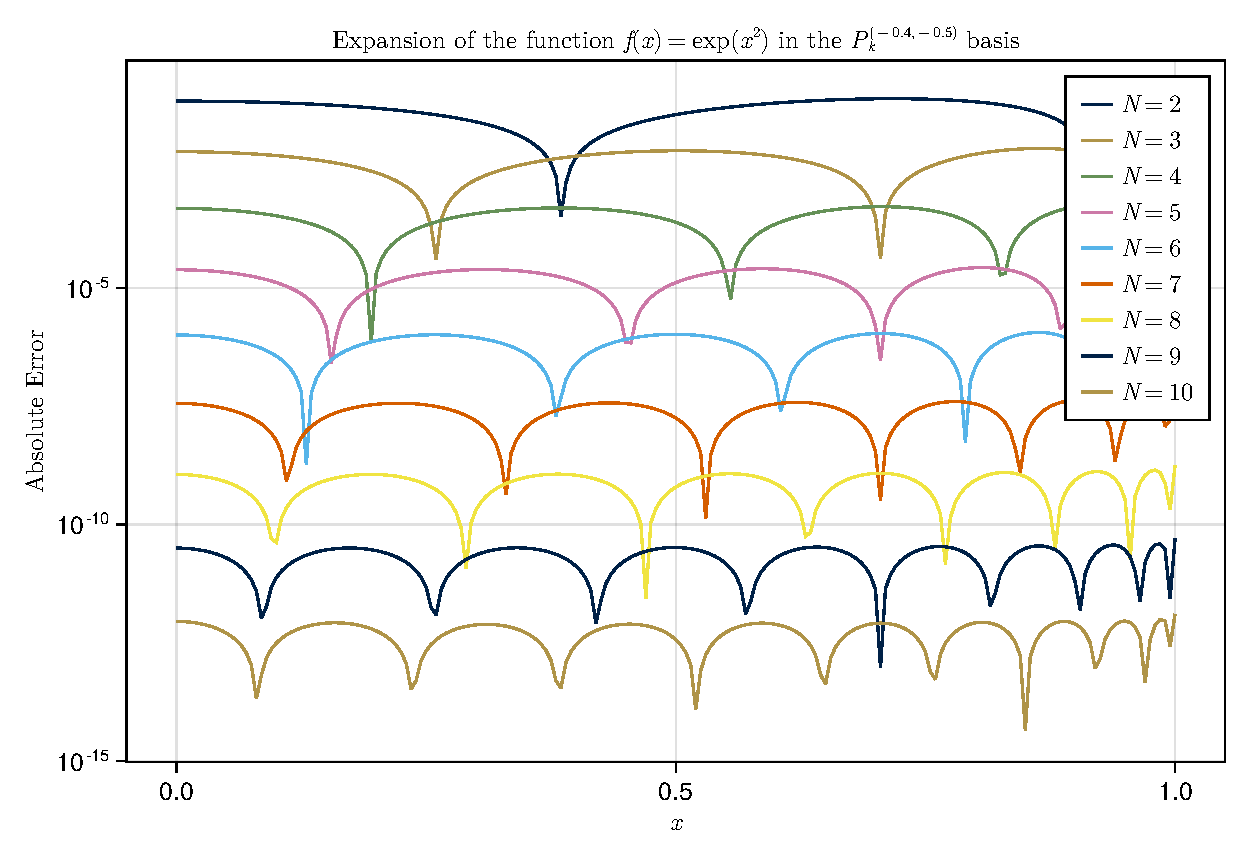
\includegraphics[width=0.7\linewidth]{results/jacobi-expansions.pdf}
  \caption[Convergence of Jacobi basis expansion]{Convergence of the Jacobi polynomial expansion $f_N(x) = \sum_{k=0}^{N-1} P_k^{(a, b)}(x)$ of an example function $f(x) = \e^{x^2}$ with $a = -\frac{3}{4}$ and $b = -\frac{1}{2}$. Each added term improves the absolute error between the function and its expansion by a factor, so we have exponential convergence. The number of ``arches'' of each solution error function, occuring from the roots of $f(x) - f_N(x)$, approximately equals the order $N$.}
\end{figure}

% TODO: Convergence speed according to theory is...?

\begin{definition}{Gegenbauer Polynomials}{gegenbauer-polynomials}
  \begin{center}\rule{0.5\linewidth}{0.5pt}\end{center}

  \hypertarget{alias-ultraspherical-polynomials}{%
    \subsection{alias: Ultraspherical
      Polynomials}\label{alias-ultraspherical-polynomials}}

  Are a special case of the Jacobi Polynomials (cf. \Cref{def:jacobi-polynomials}) and form an
  Orthonormal Basis (cf. \Cref{def:orthonormal-basis}) under the weight given by
  \[w(x)=(1+x)^\alpha\]
\end{definition}

\begin{definition}{Chebyshev Polynomials}{chebyshev-polynomials}
  Of the first kind: \[T_k(x)\] Of the second kind: \[U_k(x)\] Also have a
  {[}{[}Three-Term Recurrence Relationship{]}{]}.
\end{definition}

\begin{remark}{}{jacobi-matrix}
  The Jacobi operator is the matrix \(X \in \R^{N \times N}\) satisfying
  $$x \cdot \vec{P}^{(a,b)}(x) = \vec{P}^{(a,b)}(x) \cdot X^T\,.$$
\end{remark}

The terms in the Jacobi operator are closely connected to the three-term recurrence relationship (cf. \Cref{thm:three-term-recurrence-relationship}), even making the matrix tridiagonal.

\begin{definition}{Ansatz}{ansatz}
  $$\rho(\vec{x}) = \left(1-\norm{\vec{x}}^{2}\right)^{m - \frac{\alpha + d}{2}} \sum_{k=1}^{N} P_{k}^{(a,b)}(2 \norm{\vec{x}}^{2}-1)$$

  % Todo: - {[} {]} is it alpha or beta in the exponent of (1-y\^{}2)?
\end{definition}

\begin{definition}{Operator}{operator}
  Either the attractive or the repulsive operator can be sparse.

  Obtained using {[}{[}Theorem 2.16{]}{]}. Derivation of the exact
  row/column form on paper ( \#include in My Dissertation (cf. \Cref{def:my-dissertation}))

  \begin{itemize}
    \tightlist
    \item
          {[} {]} What does the solver look like for other kernels?
  \end{itemize}
\end{definition}

\begin{definition}{Spectral Convergence}{spectral-convergence}
  An \(N\)-point approximation \(\varphi_N\) of a function f converges to \(f\) at spectral speed if \(|\varphi_N -f|\) decays pointwise in \([-1, 1]\) faster than \(\mathcal{O}(N^{-p})\) for any \(p = 1, 2, . . .\) so \(p \in \mathbb{N}\).
\end{definition}


\begin{theorem}{Integration Theorem that needs a name}{theorem216}
  On the $d$-dimensional unit ball $B_1$ the power law potential, with power $\alpha \in(-d,2+2m-d)$, $m\in\mathbb{N}_0$ and $\beta>-d$, of the $n$-th weighted radial Jacobi polynomial $$(1-|y|^2)^{m-\frac{\alpha+d}{2}}P_n^{(m-\frac{\alpha+d}{2},\frac{d-2}{2})}(2|y|^2-1)$$ reduces to a Gaussian hypergeometric function as follows:
  \begin{align*}
    \int_{B_1} & |x-y|^\beta (1-|y|^2)^{m-\frac{\alpha+d}{2}} P_n^{(m-\frac{\alpha+d}{2},\frac{d-2}{2})}(2|y|^2-1) \mathrm{d}y                                                                                                                                                                                                                                                                                               \\
               & = \tfrac{\pi ^{d/2} \Gamma \left(1+\frac{\beta}{2}\right) \Gamma \left(\frac{\beta+d}{2}\right) \Gamma \left(m+n-\frac{\alpha+d}{2}+1\right)}{\Gamma \left(\frac{d}{2}\right) \Gamma (n+1) \Gamma \left(\frac{\beta}{2}-n+1\right) \Gamma \left(\frac{\beta-\alpha}{2}+m+n+1\right)}{}_2F_1\left(\begin{matrix}n-\frac{\beta}{2}, \quad -m-n+\frac{\alpha-\beta}{2} \\\frac{d}{2}\end{matrix};|x|^2\right).
  \end{align*}
\end{theorem}

\Cref{thm:theorem216} gives an explicit expression for the main integral
\(Q^{\beta}: L \mapsto L\), an operator from the Function Space \(L\) to the function space \(L\), we are interested in:
\[\hat{Q}^{\beta}[\rho](x) = \int_{B_1} |x-y|^\beta (1-|y|^2)^{m-\frac{\alpha+d}{2}} P_n^{(m-
  \frac{\alpha+d}{2},\frac{d-2}{2})}(2|y|^2-1) \mathrm{d}y\] which is used
to construct the Spectral Method Operator \(Q^\beta\) (cf. \Cref{def:operator}), acting on the coefficients \(\vec{\rho}\).

\section{Derivation of Operator}
Based on the {[}{[}Three-Term Recurrence Relationship{]}{]}.

One can even determine an explicit relationship between the coefficients
in the Jacobi expansion by considering the {[}{[}Jacobi Matrix{]}{]}.

Considering the operator $\hat{Q}^\beta[\rho]$ as in \Cref{thm:theorem216}, from the [[Ansatz]] $\rho(x)$ we have
$$\hat{Q}^{\beta}(x) = \sum_{k=1}^{N} \rho_{k} \int \norm{x-y}^{\beta}(1-\norm{y}^2)^{a}P_{k}^{(a, b)}(2\norm{y}^{2}- 1) \,\ddy$$


\begin{figure}[H]
  \centering
  \label{fig:attractive-repulsive}
  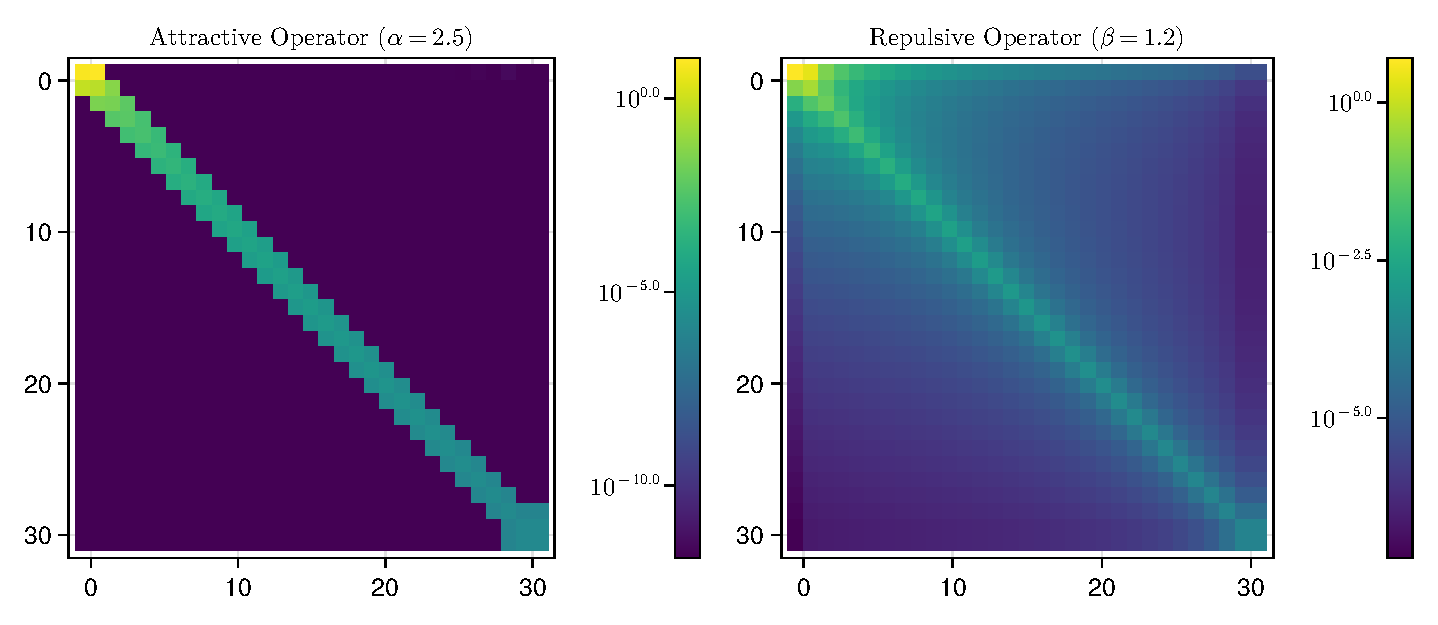
\includegraphics[width=\linewidth]{results/attractive-repulsive-operators.pdf}
  \caption[Attractive and repulsive operators.]{The attractive and repulsive operators (matrices) as given in \Cref{def:operator}, the matrix values are shown in a $\log_{10}$ color scale. Due to the choice of basis, the attractive operator is exactly banded. The repulsive parameter is only approximately banded, which the spy plots effectively demonstrate.}
\end{figure}

The bandedness of the attractive operator is due to the three-term recurrence relationship of the Jacobi polynomial basis.
% TODO.. explain

For the attractive-repulsive interaction potential, the full operator is given by
\begin{equation}
  Q_{\alpha, \beta} := \frac{R^\alpha}{\alpha} Q^\alpha - \frac{R^\beta}{\beta} Q^\beta
  \label{eq:full-attrep-operator}
\end{equation}
for some interval radius $R \in \R^+$, usually chosen as the smallest possible $R$ such that $\supp(\rho) \subseteq [-R, R]$.

\begin{figure}[H]
  \centering
  \label{fig:attrep-operator}
  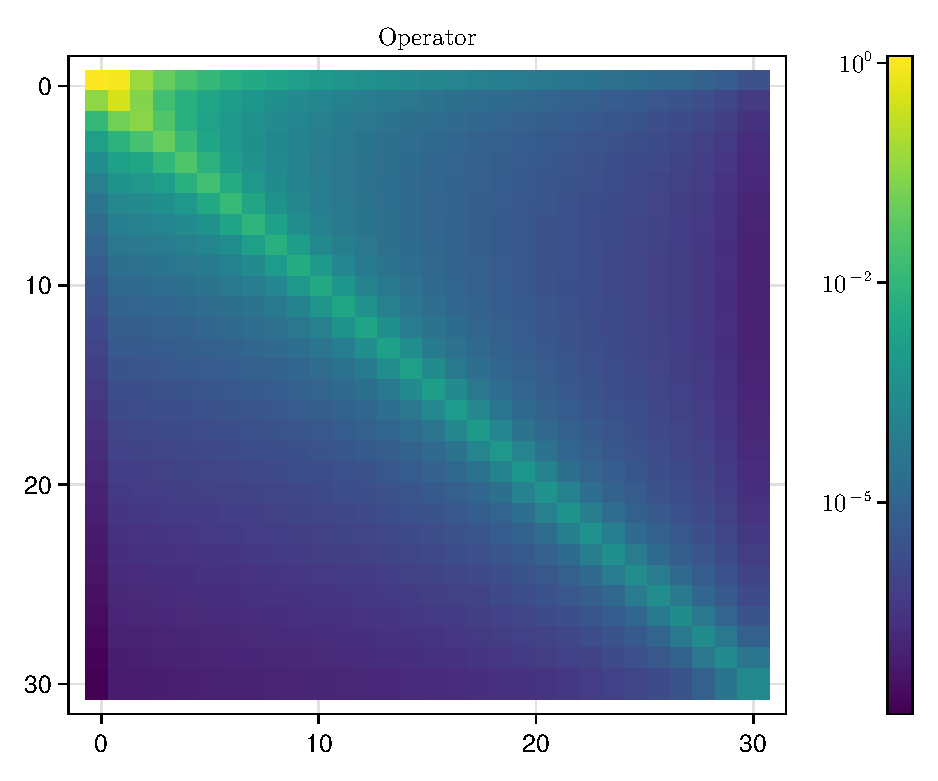
\includegraphics[width=0.5\linewidth]{results/attrep/full-operator.pdf}
  \caption[Combination of the attractive-repulsive operators]{Spy plot of $Q_{\alpha, \beta}$, the combination of the attractive-repulsive operators. Inverting this operator and applying it to $(1, 0, ..., 0)^T \in \R^N$ will yield the unnormalised coefficients $\rho_k$ of the solution expansion given in \Cref{def:ansatz}.}
\end{figure}

\section{Results}
\begin{figure}[H]
  \centering
  \label{fig:solution-increasing-order}
  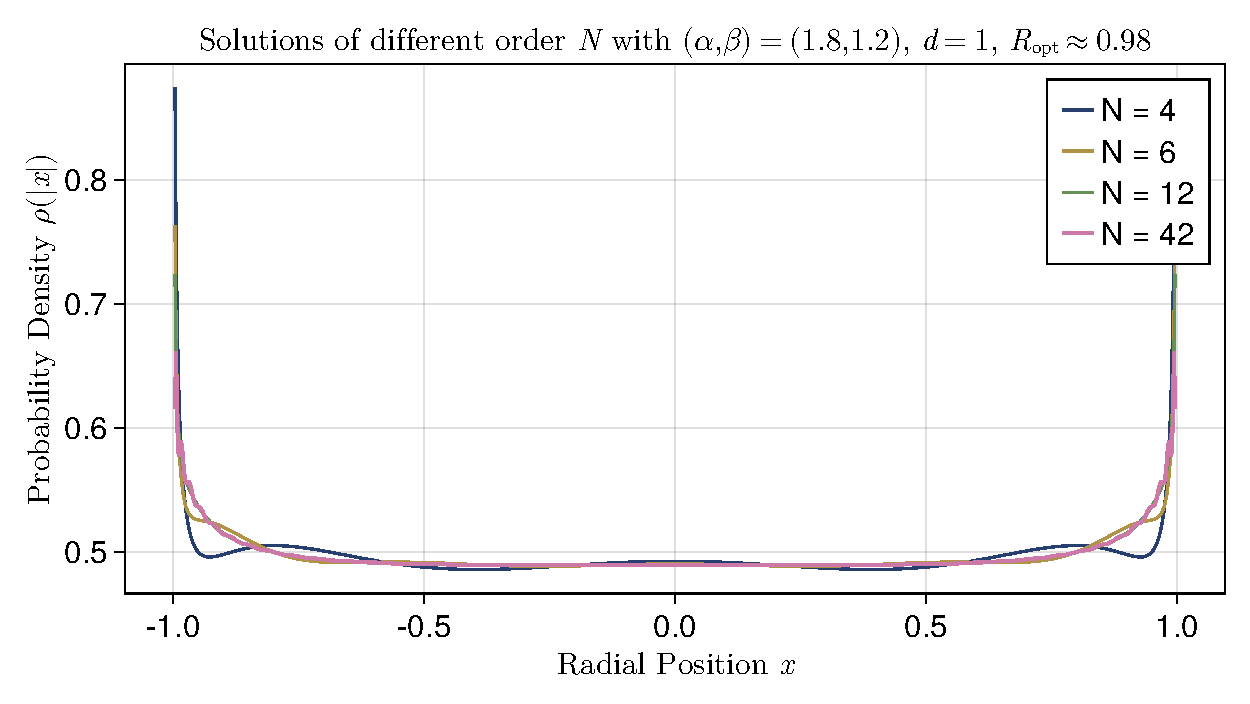
\includegraphics[width=0.8\linewidth]{results/attrep/solution-increasing-order.pdf}
  \caption[Solutions of increasing orders]{Particle density distribution function solutions $\rho$ of increasing order $N$ to the attractive-repulsive problem with interaction potential $K_{alpha, \beta}(r)$, $\alpha = 2.5$ and $\beta = 1.2$. Reflected along the y-axis for better visibility of the domain.}
\end{figure}

\section{Outer Optimisation Routine}
\begin{figure}[H]
  \centering
  \label{fig:outer-optimisation}
  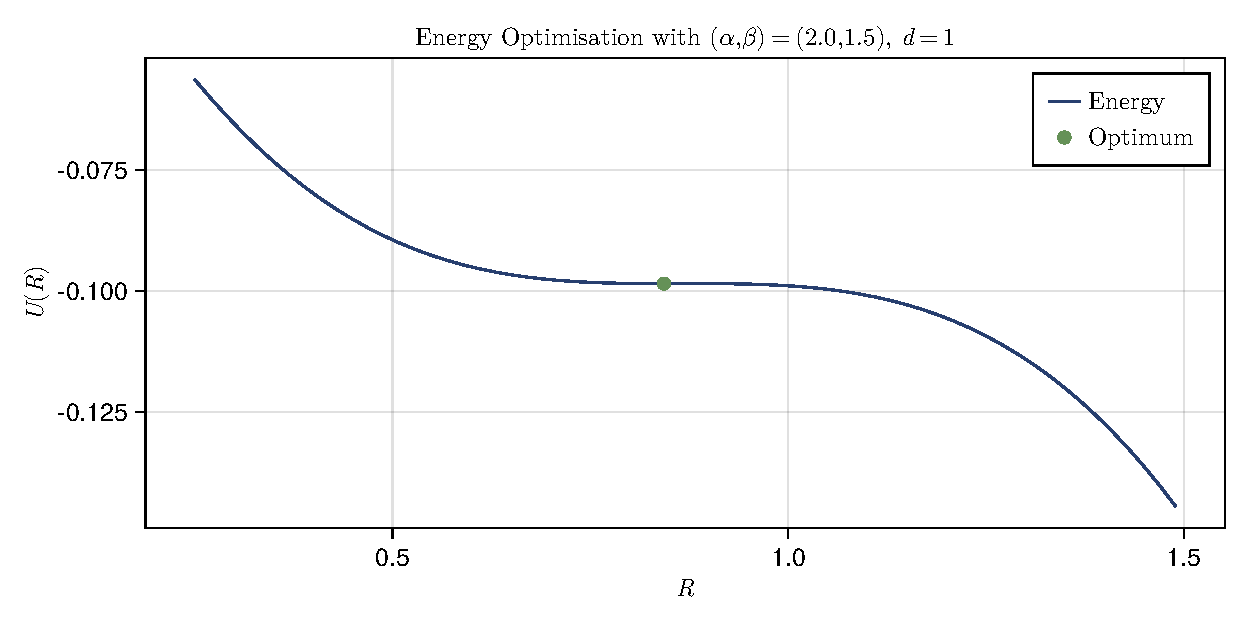
\includegraphics[width=0.8\linewidth]{results/known-analytic/outer-optimisation.pdf}
  \caption[Outer Optimisation Routine]{The total potential $U$ as a function of the support radius $R$. This is the goal function minimised by the outer optimisation routine.}
\end{figure}

Note that using this setup, the operators themselves do not need to be recomputed (cf. \Cref{eq:full-attrep-operator}).
The provided implementation uses \gls{lru} caching to automatically store operators for a given parameter set and order $N$.

\section{Comparison with Analytic Solutions}
As introduced in \Cref{sec:analytical-solutions}, there are some analytical solutions available which allow us to perform some further analysis of the numerical method in these special cases.

\begin{figure}[H]
  \centering
  \label{fig:analytic-solution}
  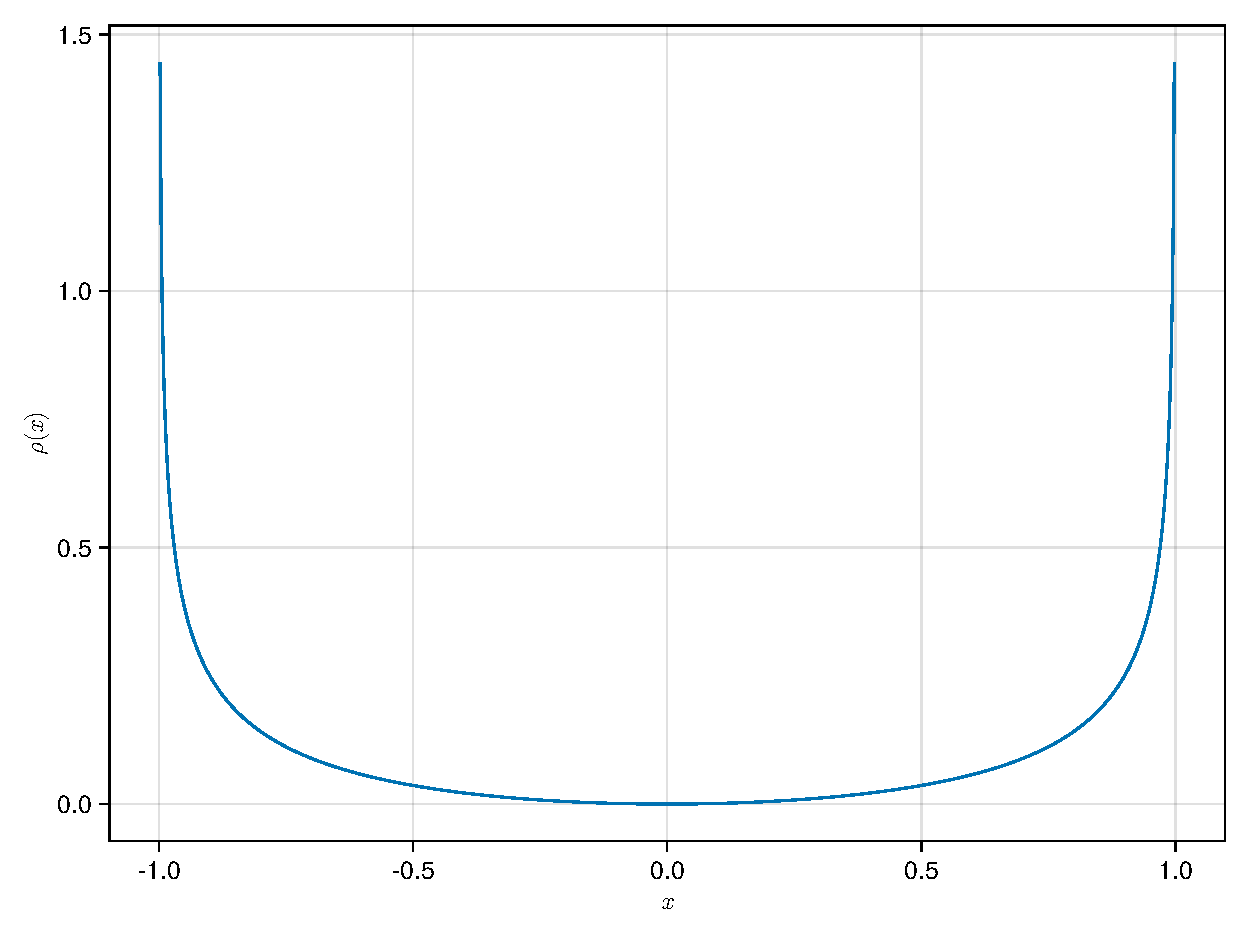
\includegraphics[width=\linewidth]{results/analytic-solution.pdf}
  \caption[Comparison with analytical solutions and error]{
    The analytic solution $\rho(x)$ given in \Cref{eq:analytical-solution-alpha-equal-2} compared to the (spectral method) solutions of different order $N$.
    The ``arches'' occur as a result of the roots of $\rho(x) - \rho_N(x)$, their number equals the order $N$ (a polynomial of order $N$ has $N$ roots).
  }
\end{figure}

\begin{figure}[H]
  \centering
  \label{fig:convergence-to-analytic}
  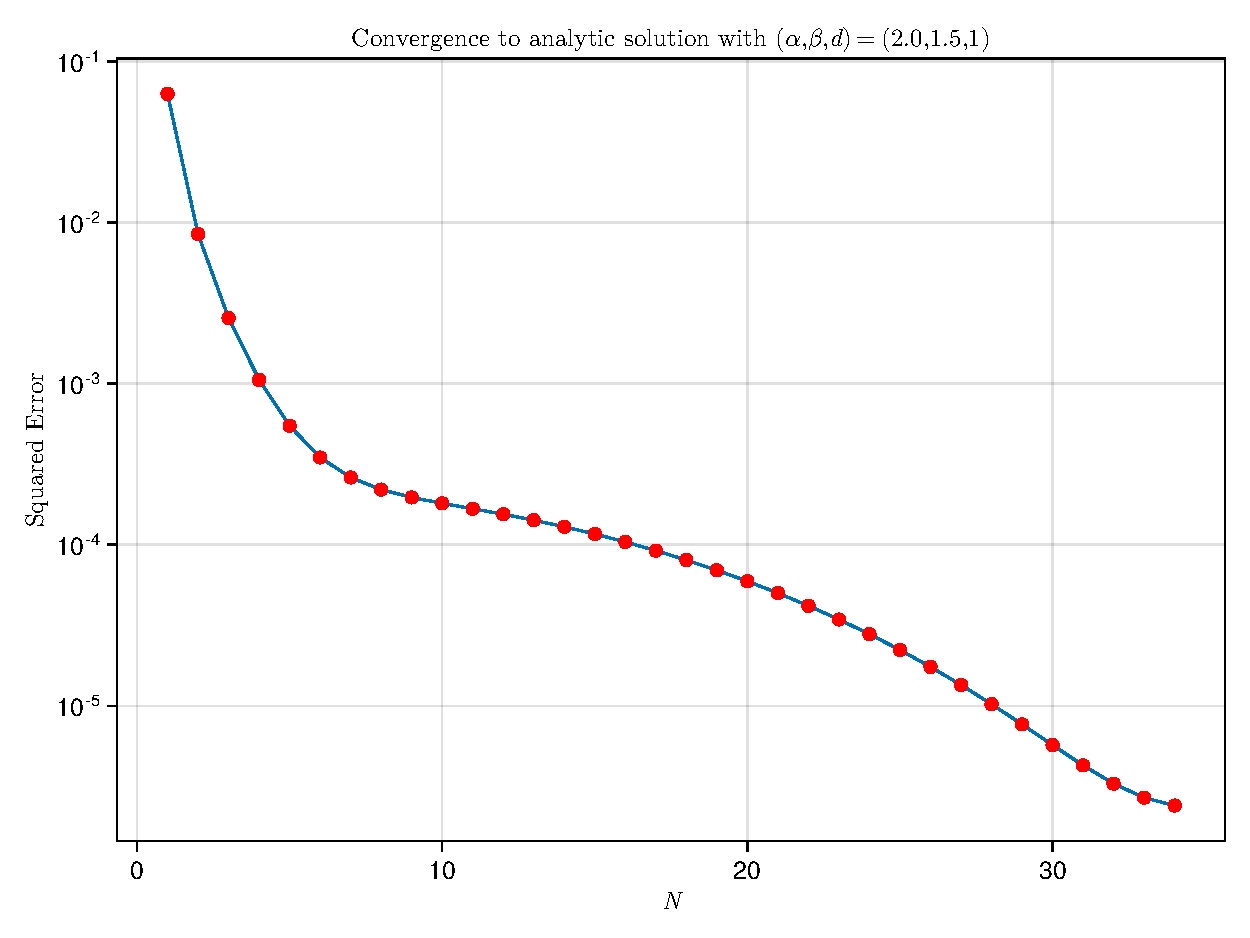
\includegraphics[width=0.6\linewidth]{results/convergence-to-analytic.pdf}
  \caption[Convergence to analytic solution]{Convergence of the numerical solution to the known analytic solution (cf. \Cref{eq:analytical-solution-alpha-equal-2}) in a special case where it is known, squared error plotted as a function of the highest order in the expansion $N$.}
\end{figure}

\section{Discussion}
\begin{figure}[H]
  \centering
  \label{fig:convergence}
  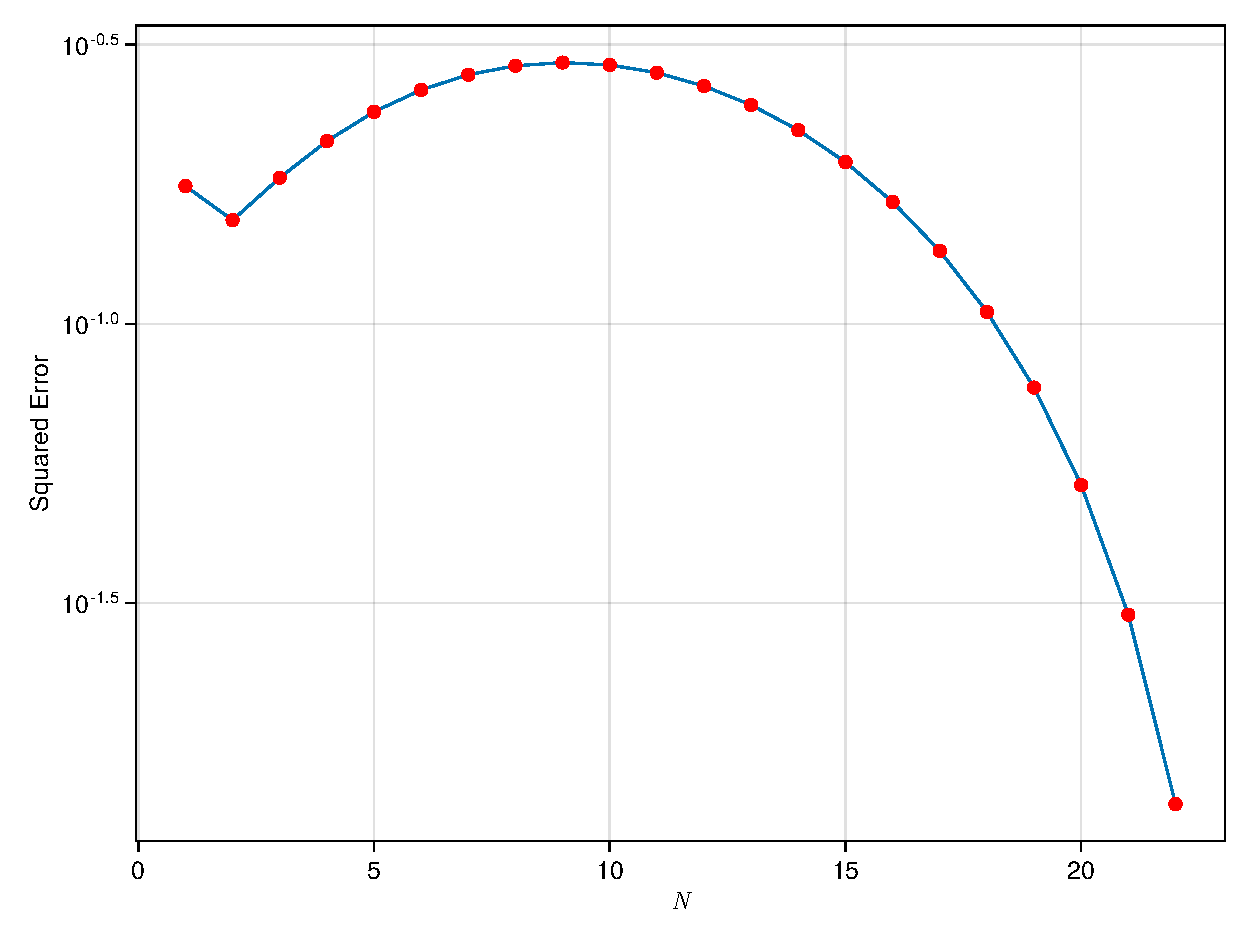
\includegraphics[width=0.7\linewidth]{results/convergence.pdf}
  \caption[Step-by-step convergence of solutions compared to order 24]{Step-by-step convergence of numerical solutions $\rho_N(x)$ as compared to $\rho_{24}(x)$, visualised using the squared error of the pointwise evaluation of both functions in $200$ points.}
\end{figure}

\begin{figure}[H]
  \centering
  \label{fig:spatial-energy-dependence}
  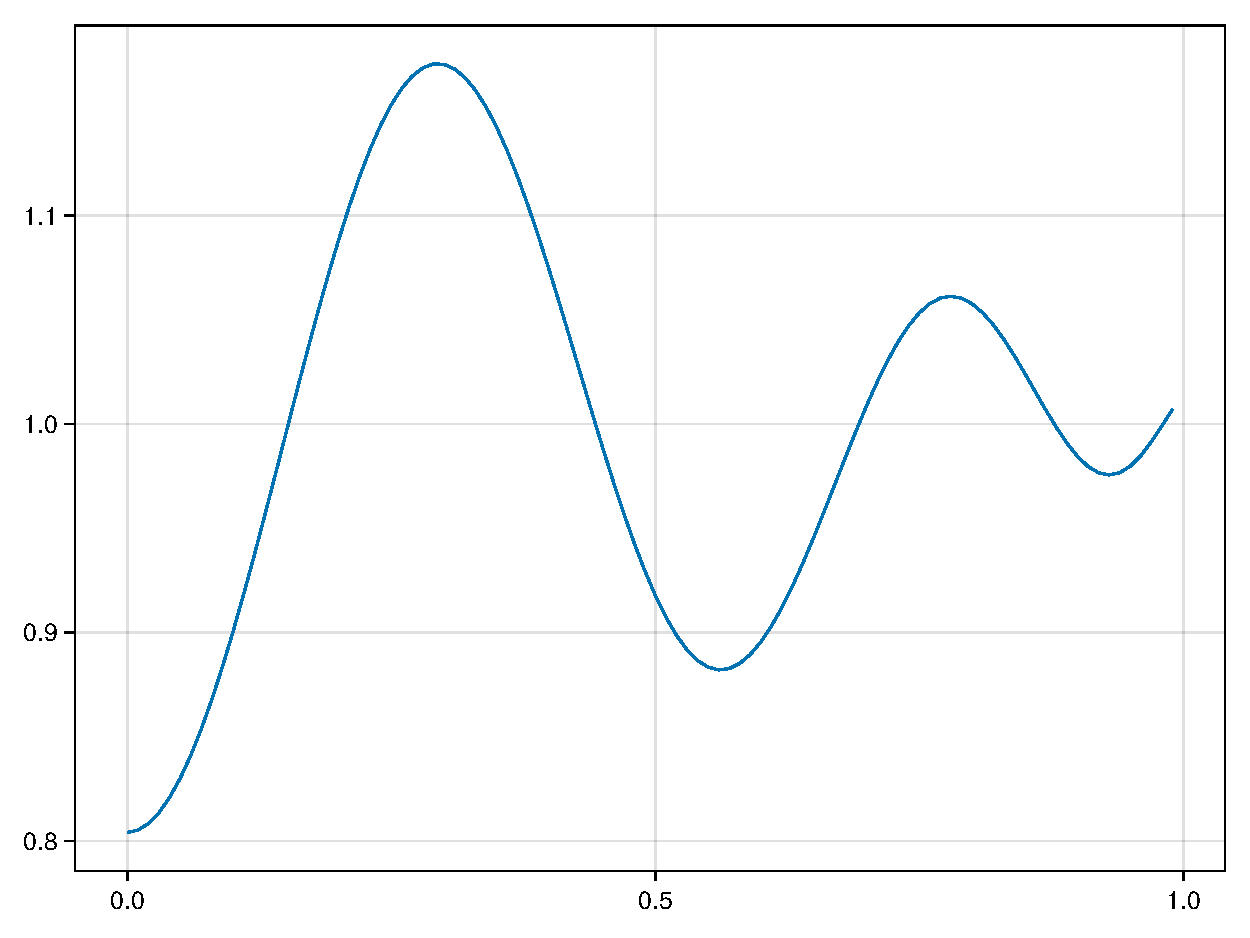
\includegraphics[width=0.6\linewidth]{results/energy-dependence-on-r.pdf}
  \caption[Spatial energy dependence on $r$]{Plot of the spatial energy dependence on $r$, for different values of the domain support radius $R$. As one can see, they are constant and this figure is only present as visual proof to increase our confidence in the construction of the spectral method.}
\end{figure}

\begin{figure}[H]
  \centering
  \label{fig:varying-parameters}
  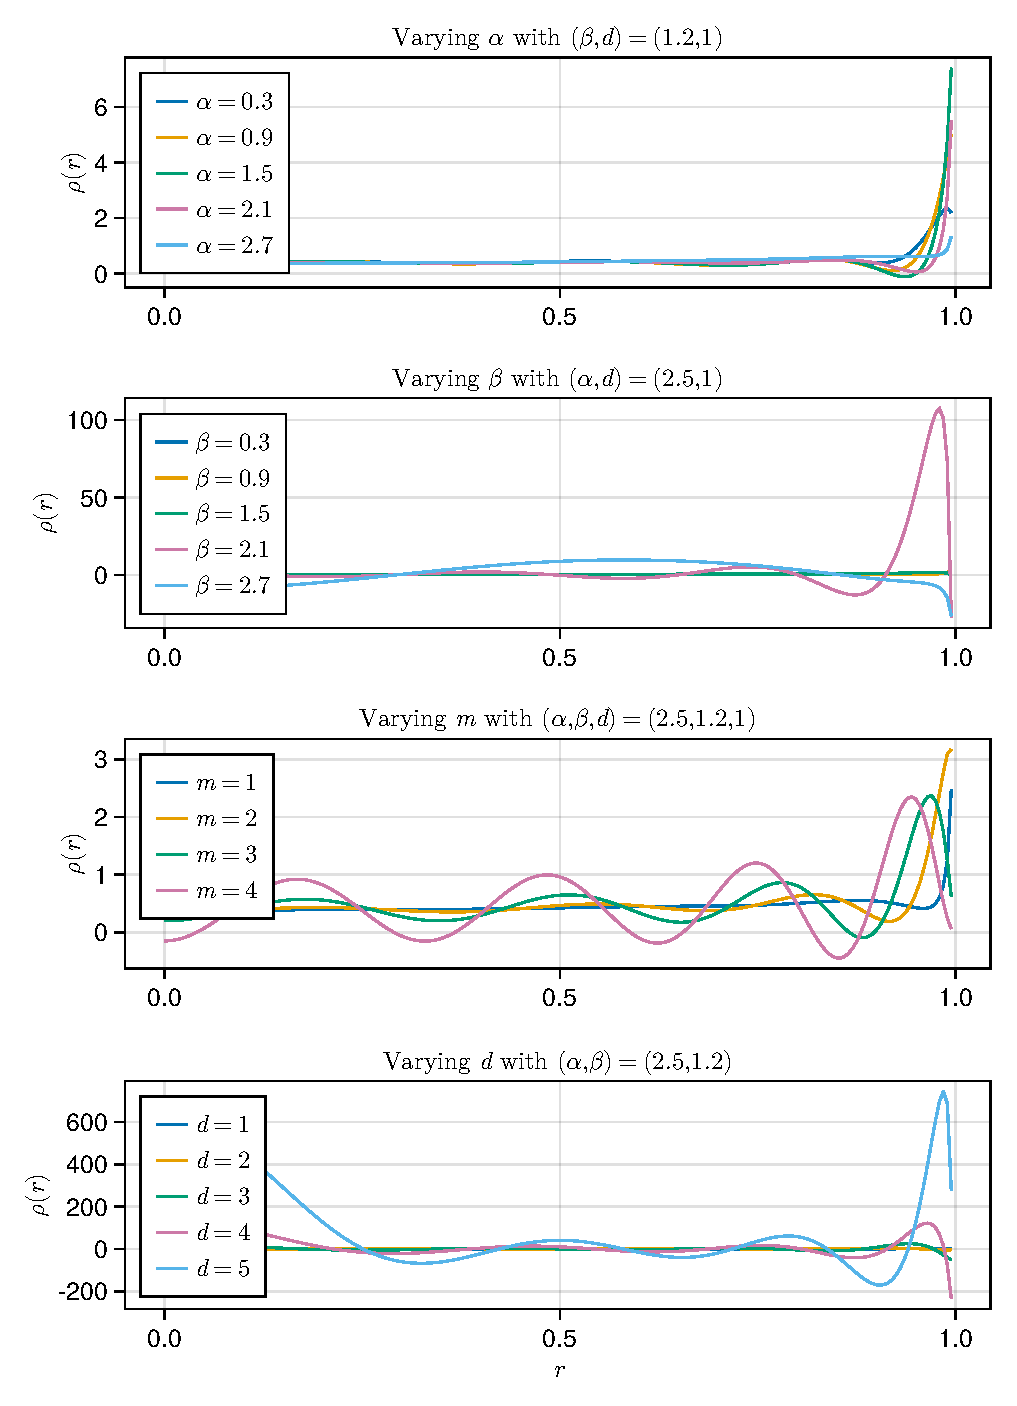
\includegraphics[width=0.9\linewidth]{results/varying-parameters.pdf}
  \caption[Varying parameters in the solver]{
    Varying different parameters in the solver to demonstrate their effect.
    See also, \Cref{fig:varying-R-solutions}.
  }
\end{figure}

  \chapter{General Kernel Spectral Method}
\label{chap:general-kernel-spectral-method}

Now that we know how to treat power law potentials in the construction of a spectral method for the solution of equilibrium measures, can we consider more general kernels as well?
The approach in this chapter will be to expand a general kernel $K$ in a power law basis and utilise the methodology introduced in the previous chapter to construct a general kernel spectral method.

\section{Expansion of the General Kernel}
More specifically, one choice of basis that could be made is the basis of monomials (so integer powers of the power law kernel basis).
Using standard methods from function approximation theory, we expand the general kernel $K: \R^+ \mapsto \R$ in the basis of $G$ Jacobi polynomials (cf. \Cref{def:jacobi-polynomials})
$$K(r) \approx \sum_{l=0}^{G-1} \tilde{g_k} P_k^{(a, b)}\left(2 r^2 - 1\right)\,, \quad \tilde{g_k} \in \R, \;l = 0, ..., G-1\,,$$
which we then reproject into the monomial basis to obtain the monomial coefficients $g_k \in \R$ such that
\begin{equation}
  K_G(r) = \sum_{l=0}^{G-1} g_k r^l \approx K(r)\,,\quad g_k \in \R, \;l=0, ..., G-1\,.
  \label{eq:monomial-expansion}
\end{equation}

\subsection{Reprojection from Radial Jacobi Polynomials}
For versatility in the choice of basis, we obtain the monomial coefficients of a given kernel $K(r)$ by
$$\vec{g} = B \tilde{\vec{g}}\,,$$
where $B \in \R^{G \times G}$.

% Does reprojection from Jacobi to monomials make sense / is it better for stability etc.?
% If so, explain reprojection using basis transformation matrix. --> yes.

\section{Description of the Method}
Given the Ansatz, the total energy of the equilibrium measure (cf. \Cref{def:equilibrium-measure}) is given by
\begin{align*}
  U_{K_G}[\hat{\rho}] & = \iint K_G\left(\norm{\hatvec{x}-\hatvec{y}}\right) \,\dd\hat{\rho}(\hatvec{x})\dd\hat{\rho}(\hatvec{y})
  = \sum_{l=0}^{G-1} g_l \iint \norm{\hatvec{x}-\hatvec{y}}^l \,\dd\hat{\rho}(\hatvec{x})\dd\hat{\rho}(\hatvec{y})                \\
                      & = R^{2d} \sum_{l=0}^{G-1} g_l R^l \iint \norm{\vec{x}-\vec{y}}^l \,\dd\rho(\vec{x})\dd\rho(\vec{y})
  = R^{2d} \sum_{l=0}^{G-1} g_l R^l U^{(l)}[\rho]\,,
\end{align*}
using \Cref{def:power-law-potential}.

The solution process then follows analogously from \Cref{chap:spectral-method}.
A spy plot of the full operator may be found in \Cref{fig:morse-operator}, resulting solutions in \Cref{fig:morse-solution-increasing-order}.

\begin{figure}[H]
  \centering
  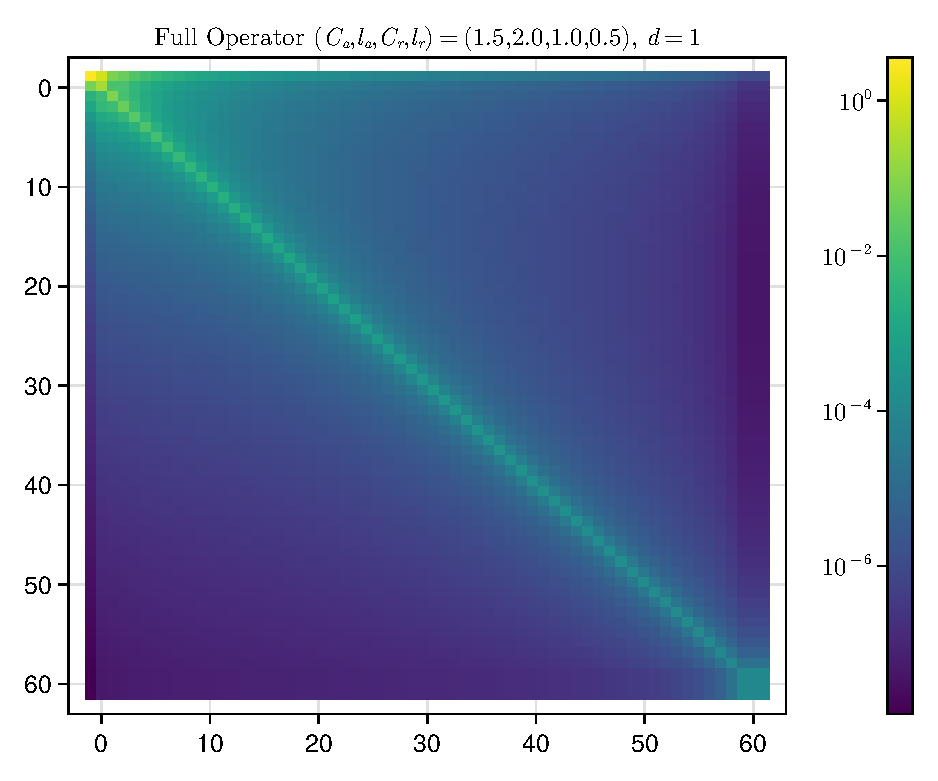
\includegraphics[width=0.5\linewidth]{results/morse/full-operator.pdf}
  \caption[Full Morse operator]{The full operator constructed from the $G=8$th order monomial expansion $K_G$ of the Morse potential function $K_{C_a, l_a, C_r, l_r}(r)$ with parameters as given above.}
  \label{fig:morse-operator}
\end{figure}

\begin{figure}[H]
  \centering
  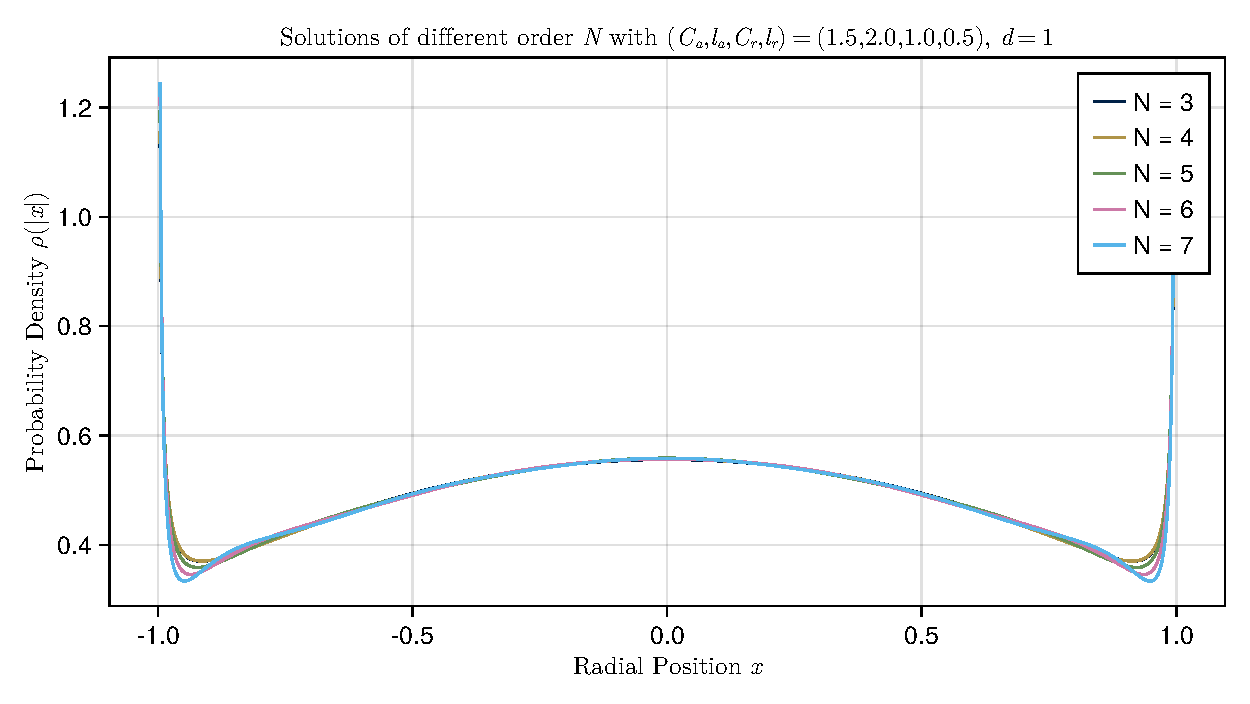
\includegraphics[width=0.8\linewidth]{results/morse/solution-increasing-order.pdf}
  \caption[General kernel solutions of increasing order]{Solutions $\rho_N(x)$ of increasing order $N$ in the general kernel setting with a monomial expansion of highest order $G = 8$ of the Morse potential $K_{C_a, l_a, C_r, l_r}(r)$.}
  \label{fig:morse-solution-increasing-order}
\end{figure}

Instead of increasing the order of the expansion in the solution ansatz (cf. \Cref{eq:ansatz}), one can increase the expansion order of the general kernel, $G$ to ensure a good match between the general kernel expansion and $K_G(r)$.

\begin{figure}[H]
  \centering
  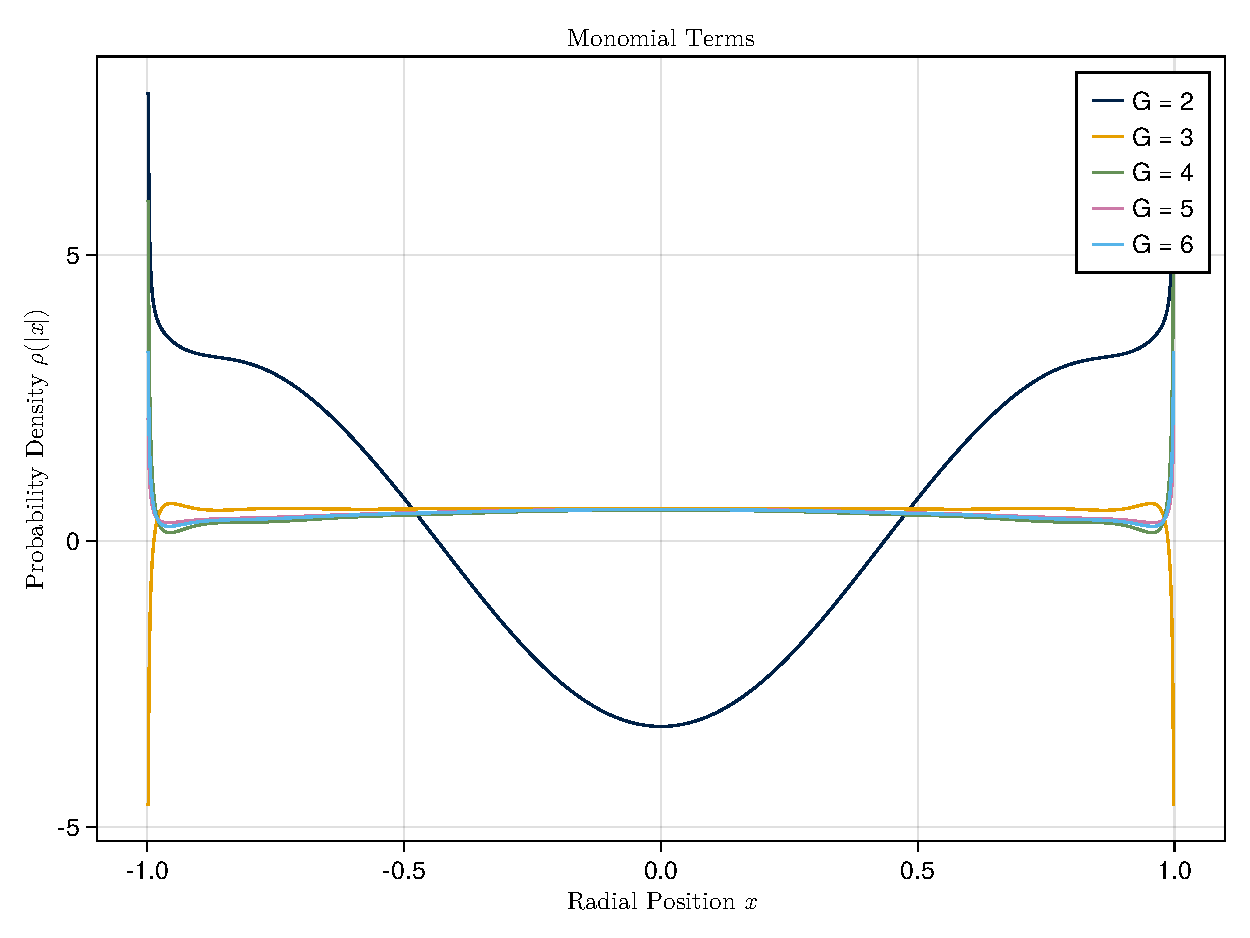
\includegraphics[width=0.8\linewidth]{results/morse/monomial-solutions.pdf}
  \caption[General kernel solutions with varying $G$]{Solutions $\rho_8(x)$ for an increasing number of terms $G$ in the monomial expansion of a general kernel $K$, in this case given by the Morse potential $K_{C_a, l_a, C_r, l_r}(r)$. So each solution $\rho_8(x)$ is a linear combination of $8$ Jacobi polynomials together with a weight, cf. \Cref{eq:ansatz}.}
  \label{fig:monomial-solutions}
\end{figure}

As one can see, the solutions improve the better the approximation of the general kernel $K$ becomes with growing order $G$ of its monomial expansion.
To make a better statement about this numerical behaviour, consider \Cref{fig:monomial-basis-convergence}.

\begin{figure}[H]
  \centering
  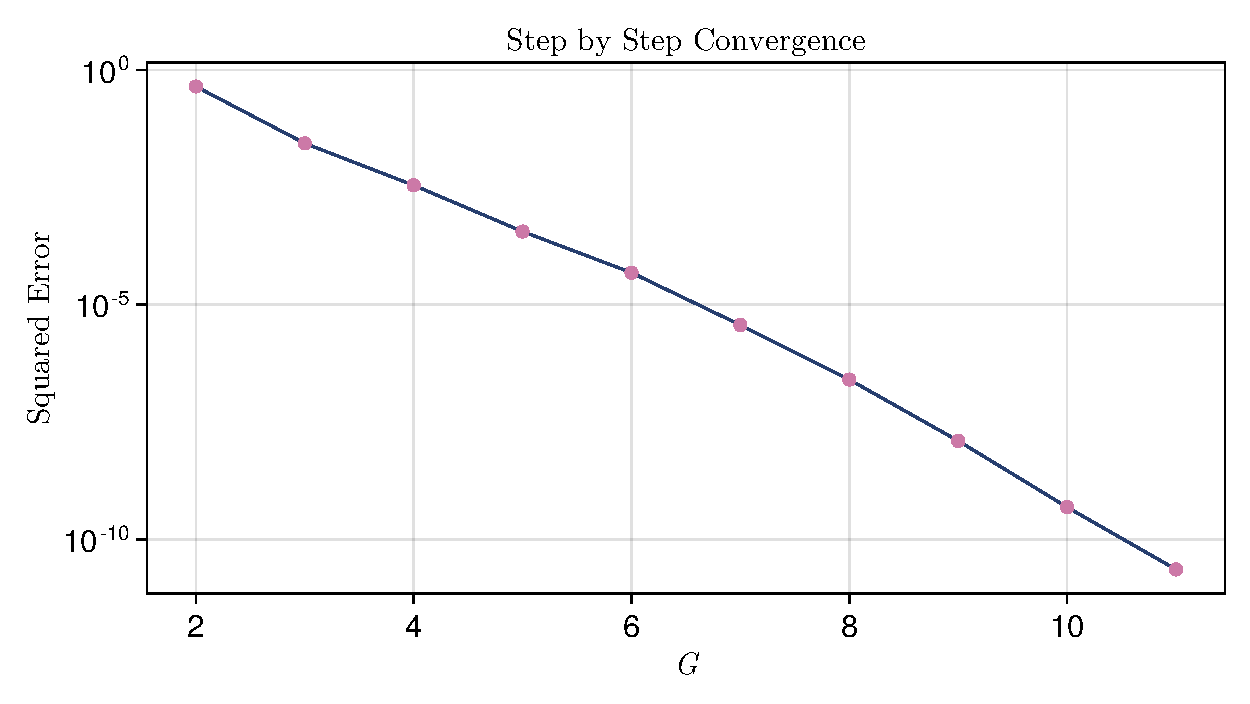
\includegraphics[width=0.7\linewidth]{results/morse/monomial-basis-convergence.pdf}
  \caption[Step-by-step convergence of solutions when increasing the degree of the monomial]{
    Convergence of numerical solutions $\rho_N(x)$ as compared to $\rho_{24}(x)$, visualised using the squared error of the pointwise evaluation of both functions in $200$ points.
    The solver again uses $K(r) = K_{C_a, l_a, C_r, l_r}(r)$.
  }
  \label{fig:monomial-basis-convergence}
\end{figure}

Solutions for varying support radius $R$ can be found in \Cref{fig:varying-R-solutions}.

\begin{figure}[H]
  \centering
  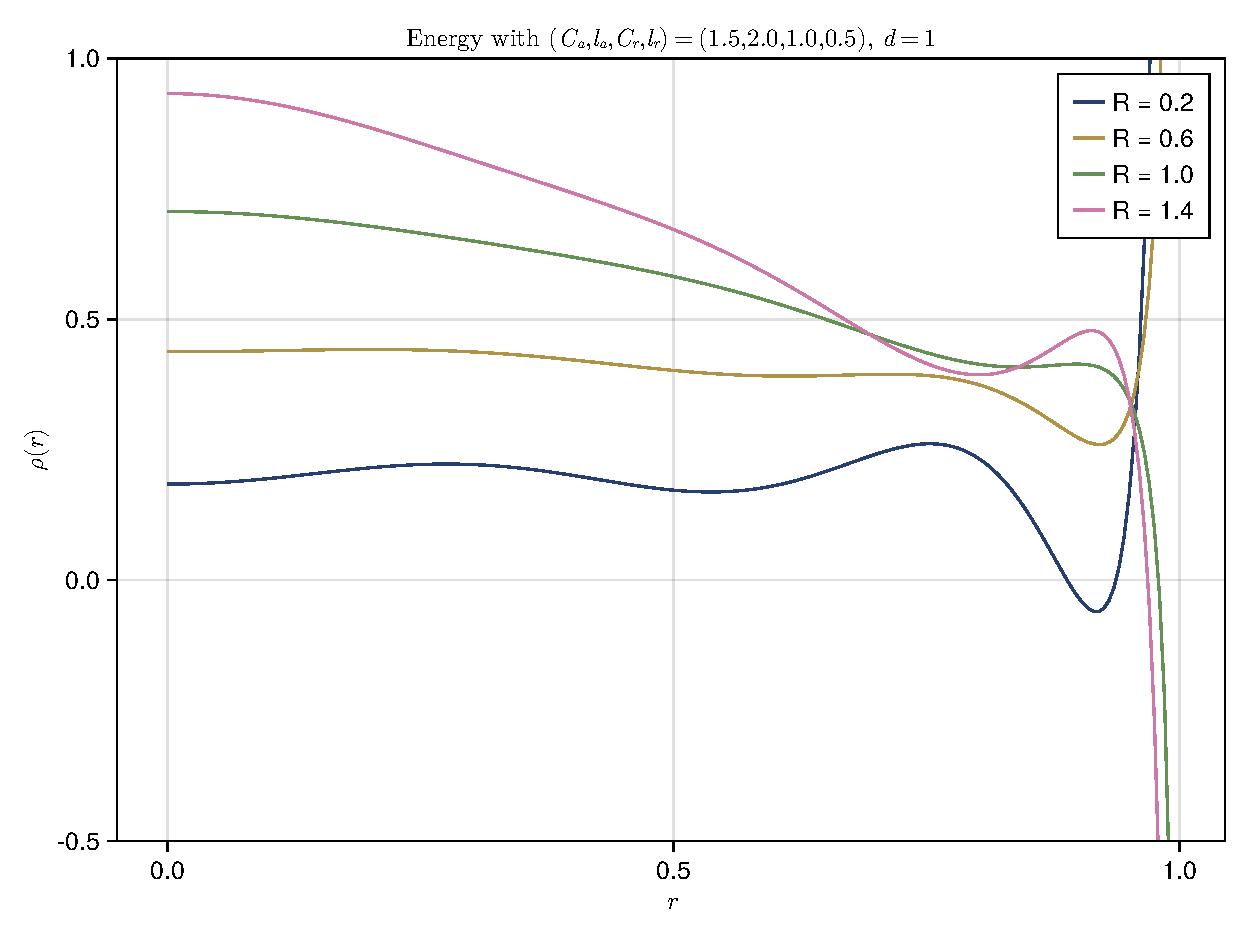
\includegraphics[width=0.7\linewidth]{results/morse/varying-R-solutions.pdf}
  \caption[Solutions with varying $R$]{General kernel solutions ($N = 6$, $G = 8$) with varying $R$ when using the Morse potential $K_{C_a, l_a, C_r, l_r}(r)$ with parameters as given above.}
  \label{fig:varying-R-solutions}
\end{figure}

Do the singularities in the solution actually exist?

  \chapter{Implementation and Results}
\label{chap:implementation-and-results}

% \input{chapters/out/Implementation and Results.md.tex}

\begin{figure}[H]
  \centering
  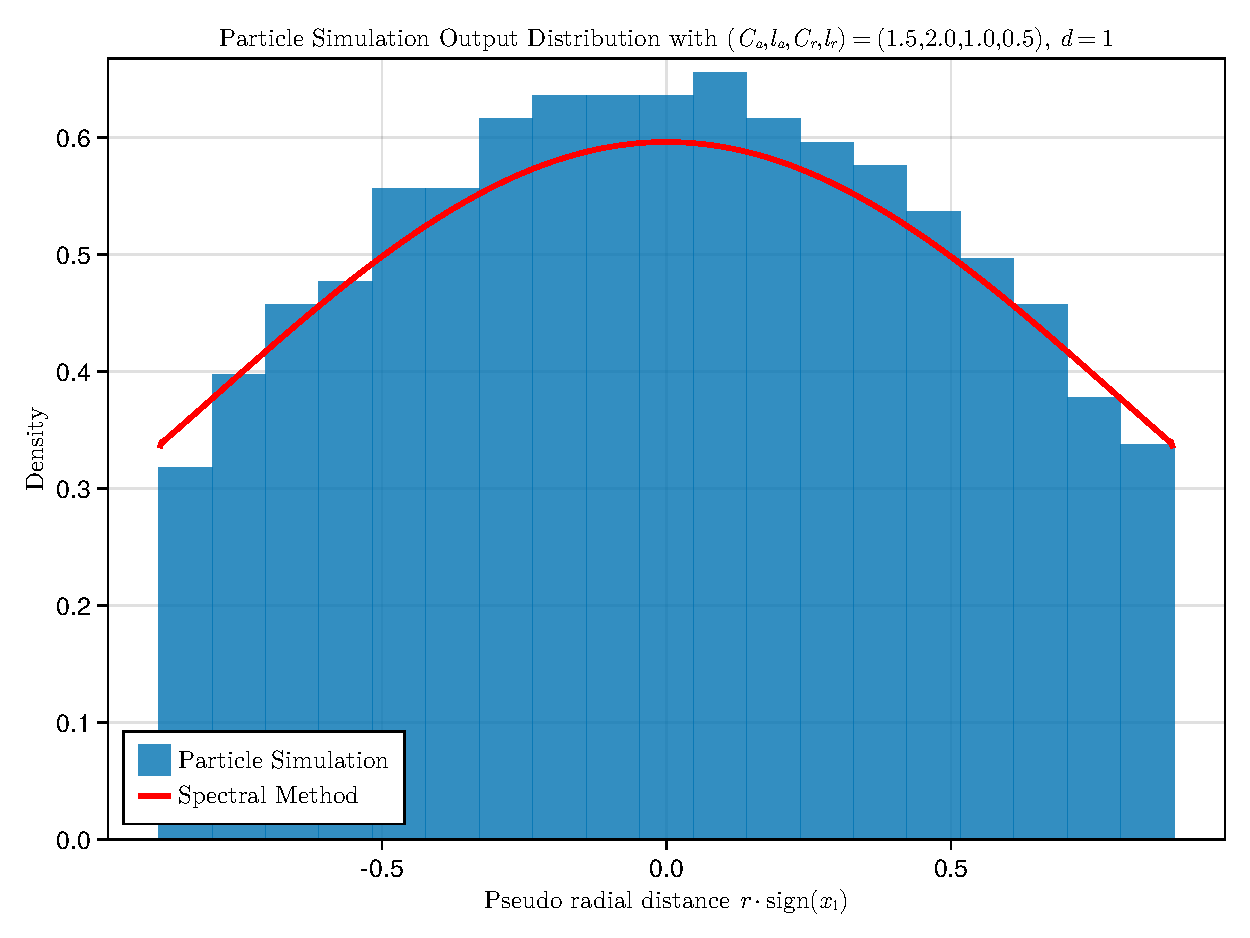
\includegraphics[width=0.8\linewidth]{results/morse/simulation-solver-comparison.pdf}
  \caption[Comparison of histogram and spectral method solution]{Comparison of the radial distance histogram from the simulation output with the $G = 8$ general kernel solvers' equilibrium measure $\rho_{12}(r)$ at $R$ given by the simulator, so without using the outer optimisation routine. The interaction potential in this example is $K(r) = K_{C_a, l_a, C_r, l_r}(r)$ with parameters given above.}
  \label{fig:simulation-solver-comparison}
  % for now
\end{figure}

\section{Further Discussion}
\subsection{Well-Conditionedness}
A common flaw of spectral collocation methods, one could think of them as the highest-order limit of finite difference schemes, is their bad conditioning behaviour.
% TODO: reference

Ideally, we would like the condition number $\kappa(Q)$ to be independent of the order $N$ to which we solve our problem. That means we want
$$\kappa(Q) := \frac{\sigma_{\rm max}(Q)}{\sigma_{\rm min}(Q)} = \frac{\norm{Q}}{\norm{Q^{-1}}} = \mathcal{O}(1)$$
and not $\mathcal{O}(N)$ or even higher orders.

\begin{figure}[H]
  \centering
  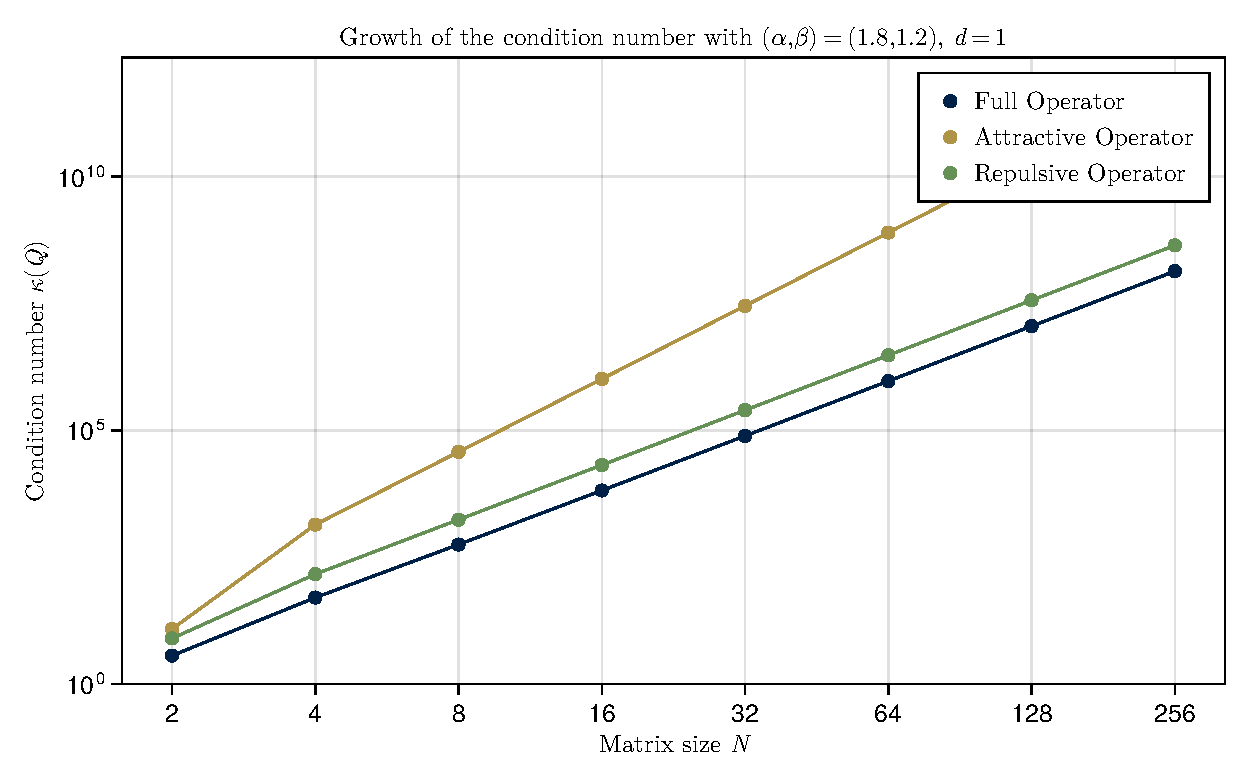
\includegraphics[width=0.8\linewidth]{results/attrep/condition-number-growth.pdf}
  \caption[Growth of the condition number]{Growth of the 2-norm condition number $\kappa(Q)$ of the attractive-repulsive operator $Q$.}
  \label{fig:condition-number-growth}
\end{figure}

\begin{figure}[H]
  \centering
  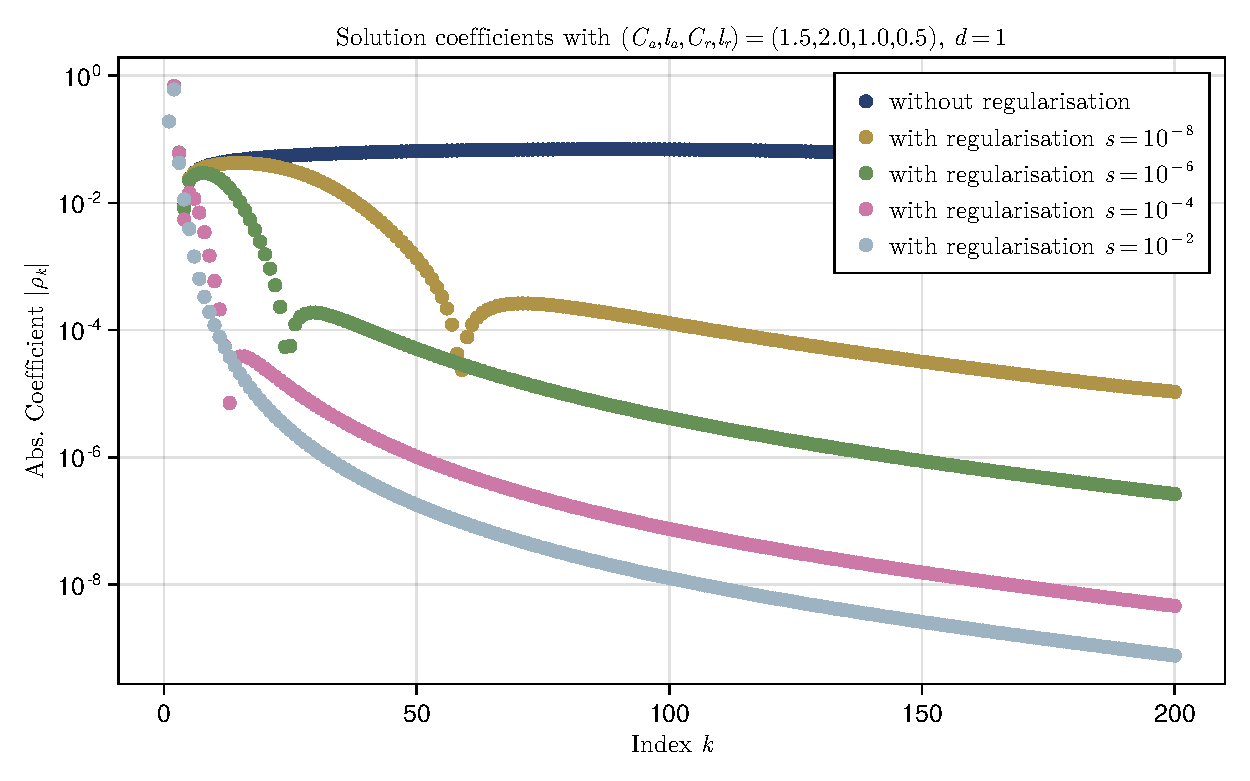
\includegraphics[width=0.8\linewidth]{results/morse/coefficients.pdf}
  \caption[Absolute value of the coefficients with and without regularisation]{Absolute value of the solution coefficients $\rho_k$ with and without Tikhonov regularisation.}
  \label{fig:coefficients}
\end{figure}

\section{Implementation Architecture}
The spectral method solver is written in Julia \parencite{2017-julia} whereas the simulator is written in C++.

To compile the simulator, please run \\
\bashblock{conan install . ----output-folder=build ----build=missing} \\
\bashblock{cd build; cmake .. -DCMAKE\_BUILD\_TYPE=Release} \\
\bashblock{make -j4}
in a bash terminal.

In order to run tests of the numerical solver implementation, run \\
\bashblock{julia solver/tests.jl} \\
in a bash terminal. In order to regenerate all plots at once, including simulation output from the C++ implementation, run \\
\bashblock{julia solver/plotall.jl}
in a terminal.

\hierKoennteIhreWerbungStehen

\section{Runtime Analysis}
\label{sec:runtime-analysis}
The following benchmarks were accumulated on an Intel\textregistered \, i7-5600U CPU running at \SI{2.6}{\giga\hertz} as the average over 3 individual runs with different test vectors, consistent across different parameter runs.
\hierKoennteIhreWerbungStehen

  \chapter{Conclusion}
\label{chap:conclusion}

% Here we summarise the work that has been presented in this dissertation and discuss possible areas for future work.

% \section{Summary}
% Give a summary of what has been done. You might do this chapter by chapter but be sure to highlight all the important points.

In the present thesis, we explored the surprisingly complex behaviour of many-body systems arising from simple pairwise particle-particle interactions and, in some cases, self-propulsion and friction terms.
For certain types of interactions, these systems approach equilibrium distributions $\hat{\rho}(\vec{x})$ which we aim to solve for using a spectral method, assuming their radial symmetry (a natural supposition in the absence of an external potential).

After introducing some theory in \Cref{chap:particle-interaction-theory} and setting up a particle simulator to verify our findings in \Cref{chap:particle-simulator}, we constructed a spectral method for power law interaction potentials in \Cref{chap:spectral-method} based on Jacobi polynomials.
The resulting spectral method is a highly efficient direct method with excellent convergence properties and solvability due to the banded operators appearing in it.
As an original extension, we introduced a numerical method for constructing the spectral solution for general kernels $K(r)$ in \Cref{chap:general-kernel-spectral-method}.
The solutions obtained by the general kernel spectral method match the results from particle simulations.
Both methods reproduce analytical solutions to arbitrary precision and provide solutions for cases in which analytical solutions are unknown.
Finally, we compared the numerical solution in the continuous situation with particle simulations in \Cref{chap:implementation-and-results}.

Next to the written part, the reader will find an implementation of the particle simulator written in C++ online \parencite{2023-my-dissertation}, including a \gls{gui}, as well as the spectral method solver written in Julia.

% \section{Future Work}
% You don't actually have to list further work, but most people do this so it seems unusual not to. Just think what you would do next if you had more time on this project.
% Other approaches, such as the one in \cite{2015-spectral-method-for-boltzmann-equation} show similar results to our spectral method.
% \hierKoennteIhreWerbungStehen

% \section{Conclusion}
% You might like to give a final conclusion so the reader is left remembering what you have done, rather than what you would do if there wasn't a submission deadline.
% This method is exponentially faster than previous techniques, requiring only minutes or seconds instead of days. Importantly, the detection time is not influenced by the system's complexity—a solution to the long-standing scalability challenge.


  \renewcommand{\glossarypreamble}{\vspace{-1cm}}
  \printnoidxglossary[type=acronym, title={Acronyms, Definitions and Theorems}]
  \thispagestyle{plain}
  \tcblistof[\section*]{def}{Definitions}
  \tcblistof[\section*]{thm}{Theorems}
  \tcblistof[\section*]{lemma}{Lemmata}
  \tcblistof[\section*]{remark}{Remarks}

  \printbibliography[heading=bibintoc]
  \chapter*{List of Figures and Tables}
  \addcontentsline{toc}{chapter}{List of Figures and Tables}
  \listoffigures
  \listoftables
  % \appendix
\titleformat{\chapter}[block]{\normalfont\LARGE\bfseries}{Appendix \thechapter \;\textendash\;}{0ex}{\vspace{-4cm}}[\vspace{4.5cm}]
\titlespacing{\chapter}{0cm}{0cm}{0cm}

\chapter{Supplemental Proofs}
\label{chap:appendix}

\end{document}
